\documentclass[lettersize]{sig-alternate-konrad}
\usepackage{listings}
\usepackage{times}  % Use Adobe Times font set
%\usepackage{epsfig,twocolumn}
\usepackage{url}
\usepackage{textcomp}
\usepackage{graphicx} 
\usepackage{color}
\usepackage{multirow}

% This will generate links within the PDF as well as a set of bookmarks
% \usepackage[colorlinks,pdfpagemode=None]{hyperref} 

%% ----- Customizations -----
\setlength{\abovecaptionskip}{-0.05in}
\setlength{\belowcaptionskip}{-0.05in}

\newcommand{\XXXnote}[1]{{\bf\color{red} XXX: #1}}
%\newcommand{\XXXnote}[1]{}

\pagestyle{empty}
%\pagenumbering{arabic}

\begin{document}

%%%%%%%%%%%% THIS IS WHERE WE PUT IN THE TITLE AND AUTHORS %%%%%%%%%%%%

\conferenceinfo{SenSys'08,} {November 5--7, 2008, Raleigh, North Carolina, USA.} 
\CopyrightYear{2008}
\crdata{978-1-59593-990-6/08/11}

\title{{\ttlfnt Lance: Optimizing High-Resolution Signal Collection
in Wireless Sensor Networks}}
\numberofauthors{1}
\author{\alignauthor Geoffrey Werner-Allen$^\dag$, Stephen
Dawnson-Haggerty$^\star$ and Matt Welsh$^\dag$\\
{\affaddr $^\dag$ School of Engineering and
Applied Sciences, Harvard
University, Cambridge, MA 02138} \\
{\affaddr $^\star$ University of California, Berkeley, Berkeley, CA 94720} \\
\email{werner@eecs.harvard.edu, stevedh@cs.berkeley.edu,
mdw@eecs.harvard.edu}
{\affaddr \texttt{http://fiji.eecs.harvard.edu/Lance}}}
\maketitle

\maketitle
\thispagestyle{empty}

%%%%%%%%%%%%%  ABSTRACT GOES HERE %%%%%%%%%%%%%%

\subsection*{Abstract}
An emerging class of sensor networks focuses on reliable 
collection of high-resolution signals from across the network.
In these applications, the system is capable of acquiring more 
data than can be delivered to the base station, 
due to severe limits on radio bandwidth and energy.
Moreover, these systems are unable 
to take advantage of conventional approaches to in-network data
aggregation, given the high data rates and need for raw signals.
These systems face an important challenge: how to
maximize the overall value of the collected data, subject to resource constraints.

In this paper, we describe {\em Lance}, a general approach to
bandwidth and energy management for reliable data collection in wireless
sensor networks. Lance couples the use of optimized, data-driven 
reliable data collection with a model of energy cost for extracting 
data from the network. Lance's design decouples resource allocation 
mechanisms from application-specific policies, enabling flexible 
customization of the system's optimization metrics.

We describe the Lance architecture in detail, demonstrating its
use through a range of target applications and resource management
policies. We present an extensive study driven by both 
real and synthetic data distributions, through simulations and runs
on a large sensor testbed.  We show that Lance maximizes 
the value of the collected data under a range of resource 
constraints, achieving near-optimal allocation of radio bandwidth and
energy. Finally, we present results from a real sensor network
deployment at Tungurahua volcano, Ecuador, in which Lance was used to
drive data collection for an eight-node network collecting seismic and
acoustic signals from the active volcano.  

%%%%%%%%%%%%%  BODY OF PAPER GOES HERE %%%%%%%%%%%%%%


\category{C.2.4}{Distributed Systems}{}
\category{C.3}{Special-Purpose and Application-Based
Systems}{Real-time and embedded systems}
\vspace{-0.1in}
\terms{Design}
\vspace{-0.1in}
\keywords{Wireless Sensor Networks, Data Collection, Resource
Management}

\chapter{Introduction}
\label{chap-intro}

An emerging application for wireless sensor networks is their use in medical
care. Many medical applications place new demands on sensor network designs.
They often involve variable data rates, multiple receivers, and mobile
nodes. Most existing sensor network designs do not adequately support these
requirements, focusing instead on aggregating small amounts of data from nodes
at fixed locations. Therefore a gap exists between existing sensor network
architectures and the requirements of medical applications.

In this dissertation, we bridge the gap by making three contributions: we
propose CodeBlue medical sensor network architecture, TinyADMR ad-hoc multicast routing protocol, and LiveNet passive monitoring infrastructure.
With CodeBlue, we address the challenges of providing a flexible 
and implementable system architecture for mote-based medical
sensor networks. TinyADMR addresses challenges in multicast routing with the
existence of low quality radio links, memory and bandwidth limitations.
LiveNet addresses the challenges for evaluating deployed medical sensor
networks by reconstructing network dynamics without introducing additional
overhead to the network. We evaluate CodeBlue, TinyADMR and LiveNet
with an indoor sensor network testbed and with a disaster drill deployment.

\section{Medical sensor networks}

The convergence of several new hardware technologies, including MEMS, low
power processors, and low power radio, has enabled a new class of computing
platform: wireless sensors. Wireless sensors combine the capability of
sensing, computation, and wireless communication into a single physical
package, enabling a wide range of applications. Over the past decade, sensor
networks research community has explored the use of wireless sensors in
military target tracking and environmental monitoring such as habitats,
forests, volcanoes, civil infrastructures, factory equipments, and home energy
usage.

One common characteristic of most conventional sensor networks is that they
are intended for deployments of stationary nodes that transmit data at
relatively low rates, with a focus on best-effort data collection at a central
base station. Although the sensor networks research community has made
tremendous progress in perfecting networking and operating system support in
this space, we argue that there is a lack of adequate architectural
support for one emerging and important application domain: medical care.

In a hospital or clinic, outfitting every patient with tiny,
wearable wireless vital sign sensors allows doctors, nurses and other
caregivers to continuously monitor the status of their patients.  In
an emergency or disaster scenario, the same technology would enable
medics to more effectively care for large numbers of casualties.
First responders could receive immediate notifications on any changes
in patient status, such as respiratory failure or cardiac arrest.
Wireless sensors can augment or replace existing wired telemetry
systems for many specific clinical applications, such as physical
rehabilitation or long-term ambulatory monitoring.

A typical scenario involves many patients wearing sensors that monitor basic
vital signs such as heart rate or blood oxygen saturation. A small number of
medical personnel are responsible for continuously monitoring the patients
using devices such as laptops or PDAs. Using the real-time information
retrieved from the network, the medical team can treat
patients who need urgent care more efficiently.


\subsection{Application requirements}

Medical sensor networks have several different characteristics than
conventional sensor network applications. The sensors are worn by patients and the
data sinks are mobile computers carried by doctors or nurses so that the nodes
in the network are not stationary. Unlike typical sensor networks, there are
likely to be more than one data sinks in the network. Nodes can also join or
leave the network dynamically. Furthermore, the data traffic pattern is
on-demand and dynamic. Different doctors may be interested in real-time status
of different groups of patients and the groups can potentially overlap. There may
also be interests for different types or resolutions of sensor data.
Conventional sensor network architectures are inadequate in such scenarios
because the system cannot assume fixed sensor queries, sampling rate and
static traffic pattern. 


%% data may have different priorities associated with it

\subsection{Resource limitation}

In addition to meeting a different set of application requirements, medical sensor
networks, as conventional sensor network systems, face the challenges from
severe
resource limitations of the low power sensor platforms. To be practical, the
sensor nodes must be light-weight, low power and low cost so that they can be
wearable, have long enough battery lifetime and be affordable. This entails
the use of low power radio and low power processor.  For example, the mote
platform, MicaZ~\cite{micaz}, that we use for our medical sensor networks has
4~KB of RAM, a 4~MHz 8-bit CPU and a low power IEEE 802.15.4 radio with
maximum transmit power at 0 dBm. The implication of such a limited platform is
that the software running on the mote cannot be overly computationally
intensive or require large amount of memory. Yet, the system must be responsive enough
to handle complex
interactions with the environment such as sampling medical sensors and
performing radio communication in time. As a result, we not only have to find
a new architecture that fulfills the application requirements, it must also be
designed carefully so that it is light weight enough to fit into the platform
but complex enough to fulfill the application demands. 

\section{Systems challenges for medical sensor networks}

We outline a set of challenges identified through the process of designing,
implementing, deploying, and evaluating a medical sensor network. First of
all, there needs to be a new network architecture to efficiently support the
type of queries and traffic patterns for medical sensor networks. Secondly,
to support the new architecture, it is necessary to provide multicast routing
capability on resource-limited sensor nodes. Third, studying a deployed
medical sensor network requires a non-trivial network monitoring infrastructure.

\subsection{A new network architecture}

In contrast to conventional sensor network applications, medical monitoring
must support a large number of patient sensors deployed in a hospital or
disaster site, a variety of data rates, and multiple mobile receiving
devices, such as PDAs carried by doctors or medics. Moreover, medical
monitoring cannot make use of traditional
in-network aggregation since it is not generally meaningful to combine data
from multiple patients. The goal is instead to efficiently deliver information
to the correct receivers. Therefore, there is a significant gap between
existing sensor network designs and the requirements of medical monitoring. 

Supporting such broad range of requirements demands a new approach to
sensor network design. To bridge the technology gap, we propose CodeBlue, an
architecture for medical sensor networks that provides a set of protocols and
services tailored for this application domain. CodeBlue includes
a publish/subscribe communication model, a rich query interface for periodic
and triggered collection of sensor data, a dynamic sensor discovery protocol,
and a programmatic external interface based on Web Services standards.
CodeBlue provides a high-level interface to the network, making it easy to
support new sensor types and applications that tie into real-time medical
sensor data.

\subsection{Multicast on resource limited sensor nodes}

By reviewing the application requirements of medical sensor networks, it
becomes clear that an ad-hoc multicast routing protocol is more adequate
than the conventional many-to-one data collection tree routing approach.
Fortunately there are existing multicast protocols designed for ad-hoc mobile
networks. However, after the attempt to implement one such protocol, ADMR, on
our resource limited sensor platform, we have discovered several challenges
that were not foreseen by the original designers. In order to achieve
acceptable packet delivery ratio, we have to use different routing metrics that
involves the use of link quality information. We have also
investigated the challenges to scale the network within the memory and
bandwidth limitations on the sensor platform.

\subsection{Deployment support}

To find out whether a design is practical for realistic use, one needs to
deploy the network and evaluate the performance in a realistic environment.
For this purpose, we have conducted a deployment study of the CodeBlue
network. It is necessary to record system behavior in order to study
the correctness and performance of the network during the deployment. Under severe
resource constraints on CPU, memory and bandwidth, it is not practical to
record such information on the sensor nodes locally or transmit the logged
information over the radio. To overcome this problem, we have designed and
built LiveNet, an entirely passive monitoring infrastructure for
reconstructing dynamics of deployed sensor networks.  LiveNet is passive and
therefore does not require changing the application code or incur any
additional resource consumption in the network. Yet, it is able provide
valuable information for evaluating and debugging the deployed network.

\section{Dissertation outline}

The remainder of the dissertation is organized as follows.

Chapter 2 considers background and related work. This chapter introduces 
existing work in sensor networks and ad-hoc networking research community that 
are related to medical sensor networks. We also provide an overview of target
hardware platforms of this thesis.

Chapter 3 presents the requirements for a large class of medical sensor
network applications and a new software architecture to meet these
needs. We first propose the CodeBlue network architecture by presenting the
system goals and overall architecture design. We then describe individual
components
to discuss the design trade-offs in detail. Our key contributions include
proposing publish/subscribe as the appropriate networking abstraction for
a medical sensor network and designing CodeBlue Query (CBQ) interface, which
provides a programmatic interface to the medical sensor network.

Chapter 4 presents our approach to achieving efficient publish/subscribe
communication in sensor networks with mobile nodes, based on the
ADMR~\cite{admr-mobihoc01} {\em ad-hoc\/} multicast routing
protocol. We first describe the challenges encountered when designing and 
implementing the multicast layer to support publish/subscribe communication 
model for CodeBlue. We identify the
challenges from unreliable wireless radio links, memory constraints and
bandwidth constraints. We also explore and evaluate different route discovery
and expiration strategies. The key contributions include two new 
routing metrics that exploit link quality information and identifying
scalability limitations from memory and bandwidth constraints.

Chapter 5 describes LiveNet passive monitoring infrastructure. This chapter 
covers the architecture of LiveNet that involves passive sniffers, trace
merging algorithm and a set of analyses that are used to analyze CodeBlue
deployments. We also present the results of an extensive validation study of 
LiveNet's performance and accuracy with a set of controlled experiments with 
an indoor testbed, MoteLab.

Chapter 6 covers implementation and detailed performance evaluation of
CodeBlue network architecture.  We present evaluation of CodeBlue both on a
sensor network testbed and with a disaster drill deployment.  The testbed
experiments evaluate CodeBlue in scalability, fairness, latency, jitter and
effect of mobility. Then we present a deployment study that was part of a disaster
drill simulating a bus accident. Using data from LiveNet, we are able to
analyze the traffic load, network hotspots, routing paths, and query yield for
this deployment.

Chapter 7 contains lessons learned from the experience of 
designing, implementing, deploying and evaluating medical sensor networks and
provide potential future research directions. 

Chapter 8 concludes.

\section{Background}
\label{evaluation-sec-background}


%\subsection{Previous work}

% Tungurahua and Reventador deployment
%Our group is one of the first to explore the use of low-power 
%wireless sensor networks for geophysical monitoring, particularly 
%on active volcanoes. Although wireless telemetry is used on 
%seismic arrays at dozens of volcanoes worldwide, such installations involve 
%large, power-hungry equipment that is not well-suited for rapid, 
%dense deployments. As a result, even many of the most most threatening 
%and active volcanoes (e.g., Mount St. Helens~\cite{malone-81}) maintain 
%networks of less than ten stations.
%One of the primary limitations of volcano seismological studies is simply
%the lack of spatial coverage on a particular volcano.  
%This is true of
%heavily-monitored volcanoes like Mt. St. Helens and Mt. Fuji as well as
%on remote locations in Ecuador.

%Our team has been collaborating for the last two years and has deployed
%two wireless arrays on volcanoes in Ecuador. Our first deployment in
%July 2004 at Volc\'{a}n Tungurahua demonstrated the proof-of-concept, 
%involving three wireless sensor nodes sampling continuous infrasonic 
%time series data~\cite{volcano-agu04,volcano-ewsn05}.  
%The sensor array transmitted continuous, real-time infrasonic signals to
%a base-station laptop via a radio modem 9~km from the deployment site.
%The network operated for 54~hours and collected data on a dozen
%eruptive events during this time. This deployment helped us to optimize
%node placement, packaging, and radio communication in a challenging
%environment. The second installation at Volc\'{a}n Reventador is the
%subject of this paper and is described in the next section.

%In this paper we focus on our second deployment in August 2005, 
%in which we deployed a larger, more sophisticated network on the 
%upper flanks of Volc\'{a}n Reventador. A previous magazine 
%article~\cite{volcano-ieeeic06} detailed the network architecture
%and an overview of the deployment itself. Briefly, the network 
%consisted of 16~nodes, each with seismometers and microphones, 
%distributed over a 3~km extent running radially from the vent. 


\section{Lance System Architecture}
\label{lance-sec-architecture}

\begin{figure}[t]
\label{lance-fig-architecture}
\begin{center}
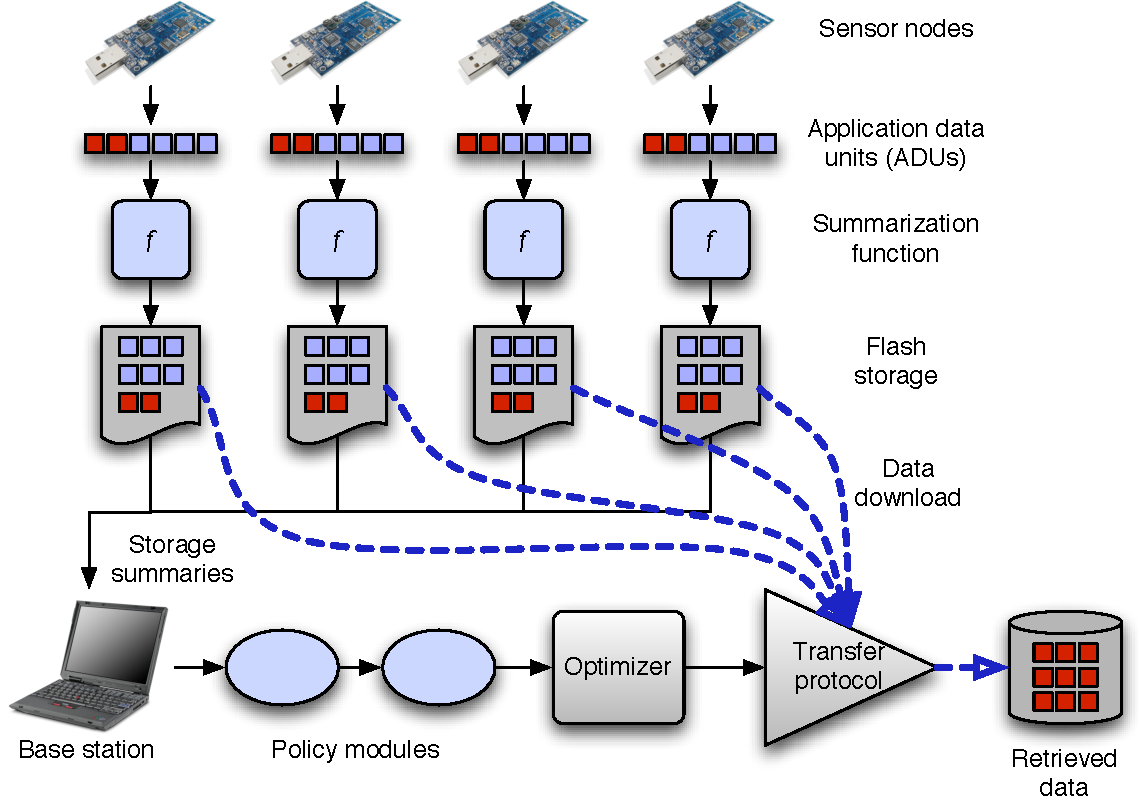
\includegraphics[width=1.0\hsize]{./4-lance/figs/new-arch.pdf}
\end{center}
\caption{\textbf{The Lance system architecture.}
The summarization portions are provided by the application; all other
components are generic.}
\end{figure}

This section describes the Lance architecture, introducing a
formal problem definition, design principles, and major system components.
Section~\ref{lance-sec-implementation} covers implementation details omitted here.

\subsection{Problem definition}
\label{lance-sec-problem-definition}

In Lance, the network consists of a set of sensor nodes that continuously
sample and store sensor data into {\em application data units (ADUs)}, which
are the unit of data storage and retrieval.  Each unique ADU $a_i$ consists
of a tuple $\{ i, n_i, t_i, d_i, v_i, \bar{c}_i \}$, 
where $i$ is a unique ADU identifier,
$n_i$ is the node storing the ADU, $t_i$ is a timestamp, and $d_i$ is the raw
sensor data.  We assume that ADUs are of uniform size and that nodes 
have sufficient flash storage to buffer collected signals, so an 
ADU is only evicted from a node's flash once it has been downloaded.
We define the {\em universe} $U$ as the set of all ADUs sampled by the 
network over time. 

Every ADU is assigned an application-specific {\em value} $v_i$ that
represents the application's intrinsic ``utility'' for the data contained
within the ADU.  We make no assumptions about how ADU values are assigned;
the value could be a function of the data itself, the time the data was
acquired, which node sampled the data, data being sampled by other nodes,
and so forth. Lance provides a flexible infrastructure for applications
to define their own value functions through policy modules.

Each ADU has an associated cost $\bar{c}_i$ that represents the energy
requirement to download the ADU from the network.  $\bar{c}_i$ is a vector
$\{ c_i^1, c_i^2, \ldots, c_i^n \}$ where $c_i^j$ represents the estimated
energy expenditure of node $j$ when ADU $i$ is retrieved. The key idea is
that we explicitly model both the energy cost for downloading the ADU from
its ``host'' node $n_i$ and the energy cost for each node along the
routing path from $n_i$ to the base station which must forward packets during
the transfer. In addition, we also model the energy cost to nodes that
overhear transmissions by nodes participating in the transfer.  This energy
cost on intermediate nodes is non-negligible, since reliable transfer
protocols involve a potentially large number of retransmission. However, the
overhearing cost is typically small, since modern low-power MAC protocols
quickly return to sleep when overhearing transmissions to another node.  The
cost vector $\bar{c}_i$ therefore depends on the network topology.

We assume that each node has a battery with a fixed capacity of $C$
joules, and no energy harvesting is performed in the field. 
Without loss of generality, let us assume that $C$ is
identical for all nodes in the network and is known {\em a priori}. 
We define the {\em lifetime target} $L$ as the desired lifetime 
of each node in the network. To meet the lifetime
target, nodes should strive to consume no more than $C/L$ 
joules per unit time on average; we call this the {\em discharge rate} of 
the node. 

The high-level goal of Lance is to download the set of ADUs that
maximizes the total value, subject to the lifetime target. Abstractly,
we define an {\em epoch duration} $\Delta$. Over each epoch, the 
energy consumption of each node must be less than the discharge rate,
that is, $\sum_i \sum_j c_i^j \leq \Delta \times C/L$. 
Determining the optimal set of ADUs to download can be determined by 
solving a multidimensional knapsack problem in which each ADU
represents an item to place in the knapsack with value $v_i$ and 
cost $\bar{c}_i$. The knapsack has $N$ dimensions (where $N$ is the
number of nodes in the network), each of size $\Delta \times C/L$
representing the energy availability over an epoch.
However, calculating the optimal
solution requires {\em a priori} knowledge of all ADUs generated by
the network over time. Clearly, any real system must make use of an
online, heuristic algorithm to approximate the optimal solution.
We discuss and evaluate several different approaches, presenting 
results with respect to the optimal offline solution.

\subsection{Design principles}

Before describing Lance in detail, we first outline several principles 
that guide its design. 

{\em Decouple mechanism from policy.}
We wish to make it easy to adapt Lance to different application
domains by providing a simple set of underlying mechanisms for 
weighing cost and data value that can be tailored 
for different
end-user goals. These core mechanisms should not be tied to any
interpretation of the data stored in an ADU. This approach leads 
to a clean separation of concerns between Lance's resource management
layer and the higher-level policies informing its operation.

{\em Simplicity through centralized control.} In a field deployment setting, 
it is highly desirable for the sensor network to be as simple
as possible, to prevent failures or unexpected behavior due to bugs.
Past deployment experiences have taught us, and others, that 
introducing complex dynamics within the network can lead to a system
that is difficult to understand, debug, or fix in the
field~\cite{volcano-osdi06,volcano-ewsn05}.
To maximize the chances of a successful deployment, 
Lance places most of the control
logic at the base station, treating sensor nodes as slave devices.
This principle makes it easy to change the behavior of the network
at the base station and allows nodes to fail independently without 
affecting the rest of the system. Conventional replication and
failover techniques can be used to bolster the reliability of the 
base station itself.

{\em Low cost for maintenance traffic.} Given limited node energy, 
we wish to reserve as much capacity as possible to support
data collection. This implies that the system
should strive to limit control messages between the base station and
the sensor nodes, as well as internal traffic within the network, as
transmitting packets unnecessarily consumes valuable energy.
This is somewhat at odds with the need for central control,
as the latter could require extensive coordination between 
sensor nodes and the base station; we wish to strike a good balance
between these two conflicting goals.

\subsection{System overview}

Figure~\ref{lance-fig-architecture} provides an overview of the Lance
architecture. Sensor nodes sample sensor data, storing the
data to local flash storage. Each application data unit (ADU)
consists of
some amount of raw sensor data, a unique {\em ADU identifier}, and a 
{\em timestamp} indicating the time that the first sample in the ADU
was sampled. ADU timestamps can either be based on local clocks at
each node, or tied to a global timebase using a time synchronization
protocol such as FTSP~\cite{ftsp}. The size of an ADU should be
chosen to balance the granularity of data storage and download with
the overhead for maintaining the per-ADU metadata. In the applications
we have studied, an ADU stores several seconds or minutes 
of sensor data, not an individual sample. ADUs are stored
locally in flash, which is treated as a circular buffer.

Ideally, nodes would be able to compute the value $v_i$ of an ADU
locally, as the data is sampled. However, since the value might depend
on factors other than the ADU's data, such as data computed at
other nodes. Lance assigns values $v_i$ at the base station,
based on global knowledge of the state of the network. However, this
requires nodes to communicate some low-bandwidth information on the ADU
contents to the base station.  For this purpose, each node applies an
application-supplied {\em summarization function}, computing a 
concise summary $s_i$ of the contents of the ADU as it is sampled.
Nodes periodically send {\em ADU summary} messages to the
base station, providing information on the ADUs they have sampled,
their summaries, timestamps, and other metadata. As a special case,
if a node is able to assign the ADU's initial value directly, this is used
as the summary.

The Lance {\em controller} receives ADU summaries from the network.
The controller also estimates the download cost $\bar{c}_i$ for each
ADU, based on information on network topology as well as a model of
energy consumption for download operations. The ADU summaries and cost
are passed through a series of {\em policy modules}, which provide
application-specific logic to assign the value $v_i$ to each ADU.
The resulting values are passed to the Lance {\em download manager}
which is responsible for performing downloads, using a reliable
data-collection protocol, such as Flush~\cite{flush-sensys07}.

\subsection{Summarization functions}

Lance computes ADU values using two application-provided components.  The
first is the summarization function, described above.  The second component
is a chain of {\em policy modules} executed at the base station which, by
modifying the value for each ADU, can implement a range of
application-specific policies. Since the base station receives ADU summaries
from every node, the policy modules can use global information not available
to individual nodes to make informed bandwidth and energy allocation
decisions.

Lance places two constraints on the on the summarization function. First,
we require that the summary be small (typically a few bytes) to limit the 
overhead for storing and transmitting these values. Second, 
the function must be able to run efficiently on the sensor node as 
ADUs are being sampled.  Otherwise, the exact form of the function is 
entirely application-specific.

As a concrete example, consider a network for downloading seismic events
from an earthquake zone.  One commonly-used measure of
overall seismicity during a time period is the Real-Time Seismic Amplitude
Measurement (RSAM)~\cite{rsam}, which computes the average amplitude
of a seismic signal over some time window (typically 1~to~10~minutes).
This function is simple to compute and reduces a complex seismic waveform
to a single scalar value, with higher values indicating greater seismic
activity.

Another form of summarization is an event detector, which would
produce a nonzero value whenever an event of interest is
contained within the ADU; the summary might also represent the strength
or confidence of the event detection. For example, an acoustic animal
tracking system~\cite{girod-ipsn07} or countersniper localization
system~\cite{shooter-localization} might use a simple trigger-based
summarization function, indicating the detection of a marmot call or
gunshot in the ADU.

\subsection{Cost estimation}
\label{lance-sec-costassignment}

Lance estimates the download energy cost
vector $\bar{c}_i$ for each ADU sampled by the network. 
We assume that nodes are organized into a spanning tree topology
rooted at the base station. The cost is a function of many factors,
including the reliable transport protocol, each node's position 
in the routing tree, radio link quality characteristics, and the 
MAC protocol. 

Given the complex dynamics that can arise during a sensor network's
operation, we opt to use a simple conservative estimate of the energy cost to
download an ADU from a node. Our approach is based on an empirical model that
captures three primitive energy costs involved in downloading an ADU. The
first, $E_d$, represents the energy used to download an ADU from a given node
which includes the energy cost for reading data from flash and sending
multiple radio packets (including any retransmissions) to the next hop in the
routing tree.  The second, $E_r$, represents the energy cost at intermediate
nodes to forward messages during the ADU transfer. The third, $E_o$,
represents the energy cost to nodes that overhear transmissions during a
transfer.  For simplicity, we assume ADUs of fixed size and compute $E_d$,
$E_r$, and $E_o$ based on the time necessary to download an ADU from the
target node.

Using this simple model, we set the elements of the cost vector $\bar{c}_i$ 
as follows. $c_i^n = E_d$ for the node $n$ hosting the ADU, and 
$c_i^m = E_r$ for nodes $m$ along the routing path from
$n$ to the base station. We set $c_i^o = E_o$ for nodes that are
assumed to be within one radio hop of any of the nodes involved in
the transfer. Estimating $\bar{c}_i$ therefore requires
knowledge of the current routing topology. This information 
is readily available: the periodic summary messages, sent to the 
base station by every node, include the node's radio neighbors and 
parent in the routing tree. Cost vectors can be easily recomputed 
whenever the routing topology changes.

To ensure that all nodes meet the lifetime target $L$, Lance models the
energy availability at each node using a token bucket with depth $D$ and fill
rate $C/L$, corresponding to the mean discharge rate.  $D$ is determined by
the target lifetime $L$, the battery capacity $B$ and the background drain
rate $R$.  In general, $D = B - L*R$, so $D$ represents the energy remaining
after the node reserves enough to ensure it can meet its target lifetime at
the background level.

\subsection{Lance optimizer}
\label{lance-sec-lanceoptimizer}

The Lance optimizer is responsible for scheduling ADUs for download,
based on knowledge of the set of ADUs currently stored by the
network, their associated values, and costs. 
ADU download itself is accomplished using a reliable transfer protocol such as 
Fetch~\cite{volcano-osdi06} or Flush~\cite{flush-sensys07}. In our
design, Lance attempts to download a single ADU at a time, in 
order to prevent network congestion, although it may be possible to
download multiple ADUs simultaneously, depending on the network
topology. A download completes either when the entire ADU has been
received or a timeout occurs.

Lance's optimization process attempts to maximize the value of the ADUs
retrieved while adhering to the lifetime target $L$. In essence, we seek a
greedy heuristic approximation of the multidimensional knapsack solution that
would be used by an oracle with complete knowledge of the ADUs sampled by the
network over all time.  The optimizer first excludes ADUs that would involve
nodes without enough energy to perform a download.  That is, if the token
bucket for a given node $m$ has $E(m)$ joules, ADUs for which $E(m) < c_i^m$
are excluded from consideration.  Note that as the bucket fills, the ADU may
become available for download at a later time. We call these ADUs {\em
infeasible}, and the remaining {\em feasible}.

To determine the next ADU to download, the optimizer considers the 
value $v_i$ of each ADU and the its associated cost $\bar{c}_i$.
We consider three {\em scoring functions} that assign a 
download score to each feasible ADU; the ADU with the highest download score
is downloaded next. In the case of ties, an arbitrary ADU is chosen.

The first scoring function, {\em value-only}, simply downloads the feasible
ADU with the highest value $v_i$. Note that {\em value-only} will meet the
network's lifetime target (since only feasible ADUs are considered) but does
not rank ADUs according to cost.  The second scoring function, {\em
cost-total}, assigns the score $\hat{v}_i$ by scaling the value of the ADU by
its total cost: $\hat{v}_i = v_i / \sum_j c_i^j$. The feasible ADU with the
highest score is then downloaded from the network. This approach penalizes
ADUs stored deep in the routing tree, which have a higher overall cost than
those located near the base station. 

The third scoring function, {\em cost-bottleneck}, scales the ADU value $v_i$ 
by the cost to the node that is an energy bottleneck for downloading
this ADU. That is, let $b$ represent the node with the minimum value
of $E(b)$ such that $c_i^b > 0$. {\em cost-bottleneck} sets the score
$\hat{v}_i = v_i / c_i^b$. The intuition behind this scoring function is
that the most energy-constrained node should be considered when
scoring ADUs for download. We evaluate all three scoring functions in 
this paper and show that they yield very different results in terms
of spatial distribution and energy efficiency.


\section{Policy Modules}
\label{lance-sec-policies}

Policy modules provide an interface through which applications can tune the
operation of the Lance optimizer. Since policy modules are loaded into the
system at the base station, they can be modified at any time without
necessitating reprogramming of the sensor nodes themselves. In this section
we provide a general discussion of policy modules and examples of policies
that can be implemented using this feature.

\subsection{Definitions}

A policy module is an application-supplied function that takes as input an
ADU $a_i = \{ i, n_i, t_i, d_i, \bar{c}_i, s_i, v_i \}$ and produces a new
ADU $a'_i$ with a possibly modified value $v'_i$. Policy modules run at the
base station, can maintain internal state, and operate with global knowledge
of the ADUs stored in the network.

\vfill\eject

A series of policy modules $\{m_1, m_2, ... m_n\}$ are composed into a linear
chain, which is passed the ADU information extracted from the ADU summary
messages received at the base station. The first policy module in the chain
is responsible for assigning the initial value $v_i$ to the ADU based on the
summary information $s_i$ calculated by the sensor node. The final ADU value
produced by the chain is used as input to Lance's optimizer for the purpose
of scheduling ADUs for download.

Lance requires that policy modules be efficient in that they can process the
stream of ADU summaries received from the network in real time. In practice
this is not difficult to accomplish, as the rate of ADU summary reception is
modest, and the base station (typically a PC or laptop) is assumed to have
adequate resources. For example, a 100-node network with an ADU size of
60~s would receive an ADU summary every 600~ms. Typical policy modules
take a small fraction of this time to run.

One of the main benefits of policy modules is that they permit significant
changes to the network's behavior \textit{without requiring changes to the
node-level summarization function}. Changing the latter would typically
involve reprogramming sensor nodes. In the field, it is often undesirable to
reprogram the network except when absolutely necessary, and in many cases it
is difficult to reach sensor nodes physically once deployed. Although systems
such as Deluge~\cite{deluge} permit over-the-air reprogramming, any changes
to the sensor node software could result in unexpected failures that can be
very difficult to debug without manual intervention. On the other hand,
introducing new policy modules at the base station is relatively
straightforward and can be quickly reversed without risking sensor node
failures.

\subsection{Example policy modules}

\begin{table}[t]
\label{lance-fig-policymodules}
\begin{center}
\begin{tabular}{|l|l|} \hline
\textit{Policy module} & \textit{Description} \\ \hline
\texttt{filter} & Set ADUs below threshold to zero value \\
\texttt{boost} & Set ADUs above threshold to max value \\
\texttt{timespread} & Dilate ADU values across time \\
\texttt{spacespread} & Dilate ADU values across space \\
\texttt{adjust} & Add or subtract offset to ADU value \\
\texttt{smooth} & Apply low-pass filter to remove noise \\
\texttt{debias} & Median filter DC debiasing \\
\texttt{correlated} & Boost values for correlated events \\
\texttt{costfilter} & Filter ADUs above cost threshold \\
\texttt{valuefilter} & Filter ADUs below value threshold \\ \hline
\end{tabular}
\end{center}

\caption{\textbf{Standard policy modules provided by Lance.}}

\label{lance-sec-example-policies}
\end{table}

Policy modules can be used to encapsulate a wide range of data collection
goals, and make it easy to customize Lance's behavior for specific
applications. We provide a standard toolkit of general-purpose policy
modules, summarized in Figure~\ref{lance-fig-policymodules}. Application
developers are free to implement their own modules as well. By composing
modules in a linear chain, it is easy to implement various behaviors without
requiring a general-purpose ``policy language.''

\begin{itemize}

\item \textbf{Value thresholding:} \texttt{filter} is perhaps the simplest
example of a policy module that filters out ADUs with a value below a given
threshold $T$ by setting their values to zero. Setting $v'_i = 0$ prevents
an ADU from being considered for download by the optimizer. This type of
filtering can be used to force a drop of low-valued data. Conversely, the
\texttt{boost} policy module sets the value for an ADU above a given
threshold to the maximum value, ensuring it will be downloaded as soon as it
is feasible.

\item \textbf{Value adjustment and noise removal:} Policy modules can be used
to remove the effects of noise or correct for node-level value bias, for
example, based on poor sensor calibration or differences in site response.
Moreover, since each node computes the ADU summary based only on local sensor
data, it may be necessary to normalize the ADU values in order to compare
values across nodes.

\hspace{0.25in} \texttt{adjust} adds or subtracts a node-specific offset to
each ADU value to correct for differences in sensor
calibration.\texttt{smooth} applies a simple low-pass filter on the raw ADU
values to remove spikes caused by spurious sensor noise. Likewise,
\texttt{debias} is intended to remove sensor-specific DC~bias from the ADU
values. \texttt{debias} computes the median ADU value for a given node over a
time window. It then subtracts the median from each ADU value before passing
it along to the next module in the chain.

\hspace{0.25in} Likewise, when a sensor network contains multiple sensors
with varying sensitivity, it is natural to prioritize data from more
sensitive instruments. In cases where networks are deployed to monitor fixed
physical phenomena, it may be desirable to prioritize data from nodes located
close to the phenomena being observed. The \texttt{adjust} module can be used
to scale raw ADU values based on a sensor's location, SNR, or other
attributes.

\item \textbf{Value dilation:} Another useful policy is to dilate a high (or
low) ADU value observed in one ADU across different ADUs sampled at different
times or different nodes. This can be used to achieve greater spatial or
temporal coverage of an interesting signal observed at one or more nodes. The
\texttt{timespread} detects ADUs with a value above some threshold $T$ and
assigns the same value to those ADUs sampled just before and just after.

\hspace{0.25in} Likewise, the \texttt{spacespread} module groups ADUs from
multiple nodes into time windows and assigns the maximum ADU value to all
ADUs in that window. Define a window $W(t,\delta)$ as the set of ADUs such
that $t-\delta \leq t_i \leq t+\delta$ where $t$ represents the center of the
window and $\delta$ the window size. \texttt{spacespread} determines the
maximum ADU in the window $v^* = \arg_{i \in W} \max v_i$ and sets $v'_i =
v^{*}$ for each ADU in $W$.

\vfill\eject

\item \textbf{Correlated event detection:} The \texttt{correlated} module is
used to select for ADUs that appear to represent a correlated event observed
across the entire sensor network. \texttt{correlated} counts the number of
ADUs within a time window $W(t,\delta)$ with a nonzero ADU value. If at least
$k$ ADUs meet this criterion, we assume that there is a correlated stimulus,
and the values for all ADUs in the set are passed through. Otherwise, we
filter out the ADUs in the window by setting $v'_i = 0$ for each ADU in $W$.

\hspace{0.25in} As an example of composing policy modules to implement an
interesting behavior, consider the chain \[
\mathit{filter}(T)\rightarrow\mathit{correlated}(k)\rightarrow\mathit{spacespread}
\] This policy filters incoming values, rejects time-correlated sets with
fewer than $k$ ADUs above the threshold, and assigns the max value across the
set to all ADUs. This can be useful in systems that wish to perform
collection of time-correlated data, but avoid spurious high-value data from a
few nodes. This policy is similar to the earthquake detector discussed in
Section~\ref{evaluation-sec-eventdetection}.

\item \textbf{Cost-based filtering:} Lance's optimizer considers both the
cost of ADUs as well as their application-assigned values when making
download scheduling decisions. The cost vector $\bar{c}_i$ is also available
to the policy module chain, allowing policy modules to perform their own
adjustments to the ADU value according to cost, permitting applications to
augment Lance's own policies for energy scheduling. For example, the
\textit{costfilter} policy module filters out ADUs with a total energy cost
$\sum_j c_i^j$ greater than some threshold; this ensures that the network
avoids expending an arbitrary amount of energy to download a given ADU
(regardless of its data value). Policy modules give applications a great deal
of control over energy usage to complement Lance's own energy scheduling
policy.

\item \textbf{Value-based filtering:} Lance's policy modules can store and
utilize history when modifying ADU values. This can be useful when \textit{a
priori} information about the expected ADU value distribution is known. For
the volcano monitoring example, traces of activity at the volcano of interest
may be available before deployment. These may be used to produce a
distribution of ADU values based on the activity levels seen during that time
period. Lance can use this distribution to decide how interesting a
particular ADU is in the context of a longer period of activity.

\hspace{0.25in} This can be particularly helpful as a way of bootstrapping
the system. Without seeding it in this way, if Lance begins running while the
volcano is quiet it will greedily begin downloading the highest-value ADUs
available despite the fact that these do not in fact contain interesting
data, wasting energy that could be saved and used later. Instead, it could
use the \textit{valuefilter} policy module with a filter threshold chosen
based on the expected ADU distribution, perhaps chosen to ADUs with values in
the top percentile. The filter threshold can also be adjusted online based on
the value distribution as ADUs are sampled.

\end{itemize}

\subsection{Interaction with ADU Summary Delivery}

The policy module chain is invoked each time a new summarization message
arrives at the base station. Once the application has assigned an initial
value, the ADU is passed to the policy module chain for processing. Note that
ADU inputs may stall along the policy module chain, or be grouped by policy
modules, so that inserting a new ADU into the chain may produce that ADU as
output, may not produce an output, or may produce a different ADU or set of
ADUs as output.

Note that policies modules like \texttt{correlated} which rely on information
from multiple nodes have to cope with delayed or missing information
resulting from dropped summarization messages. These policy modules will
usually hold sets of ADUs while awaiting members that have not yet arrived,
and then release a whole group at once after they have heard from a complete
set of nodes or a timeout occurs. When data is missing or delayed, we expect
different policy modules to respond differently. Some may choose to compute
their functions over incomplete sets of ADUs, others may not and either set
the values to zero (inhibiting download) or leave them unchanged.

Depending on the sensitivity of the policy modules in use to missing data,
different summarization message formats can be used. For our experiments we
send summarization messages each time an ADU is sampled, but which contain
the last $k$ ADU summaries (up to the maximum packet size). This ensures
that, if one is dropped, the next will contain the missing information. Other
applications may want to reduce the summarization overhead further by not
sending summarization messages each time an ADU is produced, with resulting
higher delays in policy modules like \texttt{correlated}.

\section{Adaptation to Lance}
\label{lance-sec-adaptation}

As mentioned, the Lance approach grew out of challenges emerging from our
2005 field deployment at Reventador. Although this system was successfully
deployed, it exhibited several deficiencies which led to a significant loss
of data~\cite{volcano-osdi06}.

The first problem is that the decision used to download a given signal was
based on a simplistic binary approach, based on the event-detection algorithm
running on each node. As a result, the system could not prioritize certain
events over others. The event-detector logic used a simple threshold scheme,
and as reported in~\cite{volcano-osdi06}, the threshold was set too low,
causing the network to trigger on less than 5\% of the actual seismic events.

The second problem was that following each trigger, the network initiated a
\textit{nonpreemptive} download from every node in the network in a
round-robin fashion. This policy caused the system to devote resources to
downloading small precursor earthquakes that immediately preceded larger
eruptions~\cite{volcano-osdi06}. As a result, many such larger events were
not captured.

Finally, our 2005 system made no attempt to manage energy. As a result, the
expected lifetime of the network is only about a week (using D-cell
batteries), necessitating frequent battery changes over a long deployment.
Clearly, this system could benefit from a prioritized approach to download
management that also considers energy costs to increase lifetime.

\subsection{Volcano Monitoring}
\label{lance-subsec-volcano}

To address these problems, we reimplemented our previous volcano monitoring
system using Lance. Many of the components of the original system, such as
multihop routing, time synchronization, reliable download protocol, and flash
storage interface, remained unchanged. The node-level event detector was
replaced by an ADU summarization function, as described below. The base
station code for responding to correlated events was replaced with Lance's
optimizer and policy modules. Our deployment of the completed system at
Tungurahua volcano in August 2007 is discussed in
Section~\ref{lance-sec-deployment}.

The original system was intended to detect correlated seismic events from
across the network and download data from all nodes, regardless of whether
every node detected the event. This was based on a simple event detector that
computes two exponentially-weighted moving averages (EWMA) of the seismic
signal, with different gain settings; one EWMA represents the short-term
average and the other the long-term average. When the ratio between these two
averages exceeds a threshold, an event detection message is sent to the base
station. Subsequent triggers are suppressed for a short duration afterwards.

This policy is straightforward to implement in Lance by using the ``ratio of
two averages'' as the node-level summarization function. Rather than
performing thresholding at the node level, we report the maximum ratio over
the ADU as its value, allowing Lance to prioritize different events. The base
station's policy modules are configured as shown in
Section~\ref{lance-sec-example-policies}, using a chain of \texttt{filter},
{\tt correlated}, and \texttt{spacespread} to implement the equivalent of the
event triggering policy used in the original system. Note that the Lance
version of the system differs from the original in that download management
is value-driven rather than FIFO. Also, Lance can download ADUs from
different events out of order, avoiding the nonpreemptive download problems
of the earlier system.

While our original system was designed to capture short earthquakes, were
also interested in determining whether Lance could be used to capture
different types of volcanic activity. For this, we make use of the Real-Time
Seismic Amplitude Measurement (RSAM)~\cite{rsam}, which computes the average
seismic amplitude over a given time window. Intuitively, RSAM measures the
total amount of ground shaking caused by earthquakes and tremor, and is often
used by volcano observatories to characterize the overall level of seismic
activity.

Different summarization functions and policy modules can be used to implement
a wide range of geophysical monitoring systems with Lance. For example, a
hazard monitoring system could be configured to periodically report RSAM
values for all sensor nodes and download only the strongest events for
further analysis. By limiting downloads to those ADUs with RSAM above some
threshold, energy can be saved. In contrast, a scientific study that wishes
to perform earthquake localization~\cite{aki-richards-80} or tomographic
inversion~\cite{lees-lindley-94} would prefer to download only small
earthquakes with clearly delineated onsets, which can be used to determine
the velocities of seismic waves. Likewise, a researcher studying explosive
events would prefer to download only seismic events with a corresponding
infrasonic component, since non-explosive earthquakes should not generate any
infrasound.

\subsection{Other Application Domains}

We believe that Lance can be used to benefit many applications that make use
of high-resolution signals delivered over a bandwidth-limited wireless
network. These applications require high data rates, precluding continuous
data collection, and rely on classification techniques to determine which
signals to download. Three examples follow.

\begin{enumerate}

\item \textbf{Structural monitoring:} Structural monitoring systems collect
vibration waveforms from a building, bridge, or other structure in order to
study structural properties and seismic response.  In previous
systems~\cite{netshm-emnets05,ggb-ipsn07}, data collection has been triggered
manually or on a simple periodic schedule. Instead, Lance can be used to
prioritize signals following an earthquake or forced excitation of the
structure, similar to the EWMA and RSAM functions described earlier. To save
energy, the system could choose a subset of nodes from which to download data
to achieve a good spatial distribution across the structure. The size of the
subset could be chosen depending on the strength of the excitation. In
addition, policy modules can be used to perform periodic downloading of ADUs
from each sensor for calibration, as well as to determine whether each sensor
is still functioning properly.

\textbf{Animal habitat monitoring:} Habitat monitoring applications that
deploy high-bandwidth sensors, such as microphones or cameras, are good
candidates for prioritized data extraction.  An example application may
attempt to download interesting audio signals facilitating offline species
classification or localization~\cite{girod-ipsn07}. The summarization
function could involve either a triggered event detector, an audio waveform
classifier, or motion detector from a series of camera images~\cite{cyclops}.

At the base station, policy modules can use offline knowledge of node
positions to modify the initial ADU value. One approach might enhance spatial
coverage by prioritizing data collection from nodes nearby the source of the
signal. Another could reject noise by deprioritizing signals detected by only
one node. For example, if fewer than three nodes report an audio event, it is
impossible to perform acoustic localization and Lance need not waste
bandwidth on the signal.  Policy modules can take other metrics into account
as well, such as the SNR of the recorded signal or the time of day (e.g.,
reducing confidence in camera images taken at night).

\item \textbf{Medical monitoring:} Another application domain that we are
exploring is motion analysis of patients with movement disorders, such as
Parkinson's Disease~\cite{parkinsons-embs07}. In this context, up to ten
sensor nodes equipped with triaxial accelerometers and gyroscopes are placed
on the patient's limb segments (two each on the arms and legs plus one each
on the torso and waist), collecting high-resolution data at rates up to
100~Hz or more. The goal is to capture data from the body sensor network
during periods of dyskinesia (abnormal movements) or bradykinesia (slowness
of movement) associated with the disease. The base station will typically be
a laptop located in the home, and as such will experience a wide variation in
bandwidth to the body sensor network (including disconnections), depending on
the patient's location.

Use of low-power wireless sensors keeps the size and weight of each device
down: for example, the wearable sensor node described
in~\cite{parkinsons-embs07} measures $44 \times 20 \times 13$~mm and weighs
just 10~g.  While the sensor network is not spatially distributed, and all
nodes are within a single radio hop of each other, the data rates greatly
exceed the radio channel bandwidth: a single node will consume more than a
quarter of the best-case radio capacity, assuming no protocol overhead or
retransmissions.

Following our deployment at Tungurahua Volcano in 2008 we adapted the Lance
system to support this medical monitoring application, resulting in a system
called Mercury~\cite{mercury-sensys09}. Mercury makes use of Lance to drive
the energy and bandwidth management. Each sensor node computes a series of
high-level \textit{features} from the raw sensor data, such as peak
amplitude, maximum entropy, and RMS. The node prioritization function assigns
higher priority to features appearing to represent abnormal movement. The raw
signal is also stored as separate ADUs with lower priority than the features,
allowing Lance to restrict downloads of the raw data to periods with a strong
radio link to the sensors. During periods of disconnection, nodes will buffer
ADUs for later transmission; the wearable sensors we are using support a
large (up to 2~GByte) flash memory for this purpose. Policy modules at the
base station estimate the available bandwidth to the body sensors, based on
radio link quality, and prioritize downloads accordingly.

\end{enumerate}

\section{Prototype Implementation}
\label{sec-implementation}
\label{sec-implementation-nsm}

We have implemented Lance in TinyOS 2.x~\cite{tinyos-asplos00} for 
TMote~Sky and iMote2 sensor nodes. The TMote~Sky features a
1~MB flash memory (ST~M25P80) divided into 16~sectors of 64~KB each.
Our current prototype matches the ADU size to the sector size to
simplify storage management, but this is not a fundamental limitation
in the design. Sensor nodes participate in a multihop spanning-tree 
protocol rooted
at the base station; we use the Collection Tree Protocol provided with
TinyOS~2.0 for this purpose. Nodes send a periodic storage summary to the
base station. To improve reliability, we use a
sliding window approach in which each summary includes information on
the last 5~ADUs recorded by the node. The node prioritization function
is implemented as an application-supplied NesC component conforming to
a simple API. Our prototype uses our own Fetch~\cite{volcano-osdi06}
reliable transfer protocol, although it would be straightforward to
replace this with another protocol such as Flush~\cite{flush-sensys07}.

The Lance download manager runs at the base station and receives
data from the network via a ``gateway node'' connected to the base
station by a serial cable or radio modem.  The download manager is 
implemented in Perl and makes use of several external utilities for
reading and parsing storage summary packets and sending download
requests to the network. Policy modules are implemented as separate
UNIX processes (which can be in any language; we typically use Perl) 
that read storage summaries on {\tt stdin} and produce modified
storage summaries on {\tt stdout}. A simple configuration script is
used to compose multiple policy modules into a pipe. We find that
using standard scripting languages and UNIX utilities makes it very
easy to implement a range of policy modules.
A suite of Python utilities for logging, data visualization, and 
managing the network through a GUI are also provided.

\section{Evaluation}
\label{idea-sec-evaluation}

To evaluate IDEA, we built and tested the energy-aware component and
application described in Section~\ref{idea-sec-casestudies}. For the routing
protocol, we compare our IDEA-based implementation to an approach that is not
energy-aware. For the application, we use IDEA to implement several energy
objective functions and compare their performance against each other and
against a heuristic that does not consider energy availability.

\subsection{Experimental Setup}
\label{idea-subsec-experimentalsetup}

Throughout the evaluation we present results run in several different
environments. We have implemented IDEA for TinyOS in order to run experiments
on MoteLab~\cite{motelab}, our 180~node wireless sensor network testbed. We
also present results obtained using TOSSIM~\cite{tossim}, the TinyOS
simulator. TOSSIM incorporates a closest-fit pattern matching noise model to
accurately capture complex link dynamics~\cite{cpm-ipsn07}. TOSSIM allows us
to run longer experiments incorporating various solar charging models. To
improve the realism of TOSSIM we began with a modified version developed for
the Koala project~\cite{koala-ipsn08} and performed further modifications to
correctly simulate the operation of low-power listening
(LPL), which is important to properly model the power
consumption of the radio for the ICTP experiments. We use information
collected on MoteLab to build a realistic TOSSIM radio model for our
simulations. Finally, for the application we built a Python simulator to
allow rapid prototyping of various energy objective functions.

IDEA is designed to tune components in the face of variations in both load
and charging rates, and to test this we present experiments using solar
charging data collected off of a solar panel deployed on an Arlington, MA
rooftop in March, 2009. Battery levels are calculated using a charging model
based on a Nickel-Metal Hydride battery technology with a 66\% charging
efficiency. We attenuate this data to simulate the charging produced by solar
panels of several different sizes in order to evaluate IDEA's performance as
available energy changes. We also perform experiments with a randomly
attenuated charging profile to simulate bad solar panel placement or
obstacles to incident sunlight effecting the spatial distribution of
collected energy.

For our MoteLab experiments we determine the system's ability to span periods
without charging inputs. We use two sets of initial conditions based on the
interaction between the charging data we collected and the capacity of the
batteries deployed. If the solar panel is large enough it will provide
considerable charging input and completely charge small batteries during the
day, so that all nodes begin the night with full batteries. If the solar
panel is not large enough to completely charge the batteries nodes will begin
the night with varying amounts of charge depending on their load rates during
the day.

Energy tracking is done by IDEA using a software-only approach developed for
the Pixie~\cite{pixie-sensys08} project. The component captures state
transitions and applies an energy consumption model for each state based on
current consumption measured offline. In the future we would like to
integrate a more accurate hardware-driven approach such as
iCount~\cite{icount-spots08}. The short lifetimes for some experiments are
explained by the use of extremely small batteries, which were chosen to allow
experiments to complete in reasonable amounts of time. We expect that
application developers will want to use a battery size and charging
technology suitable to allow their system to achieve a desired level of
performance, and the improvements in energy efficiency possible using IDEA
will allow smaller batteries or solar panels to be used, reducing the size
and cost of the hardware package.

Experiments for the energy-aware routing case use the first-node death energy
objective function described in
Section~\ref{idea-subsec-energyobjectivefunctions}, and therefore we evaluate
the network lifetime as the time at which the first node runs out of energy.
Our distributed localization application illustrates the process of designing
an effective energy objective function when the overall goal of the system is
known.

\subsection{ICTP: Energy-Aware Routing}

\begin{figure}[t]
\begin{center}
\textbf{(a)}\\
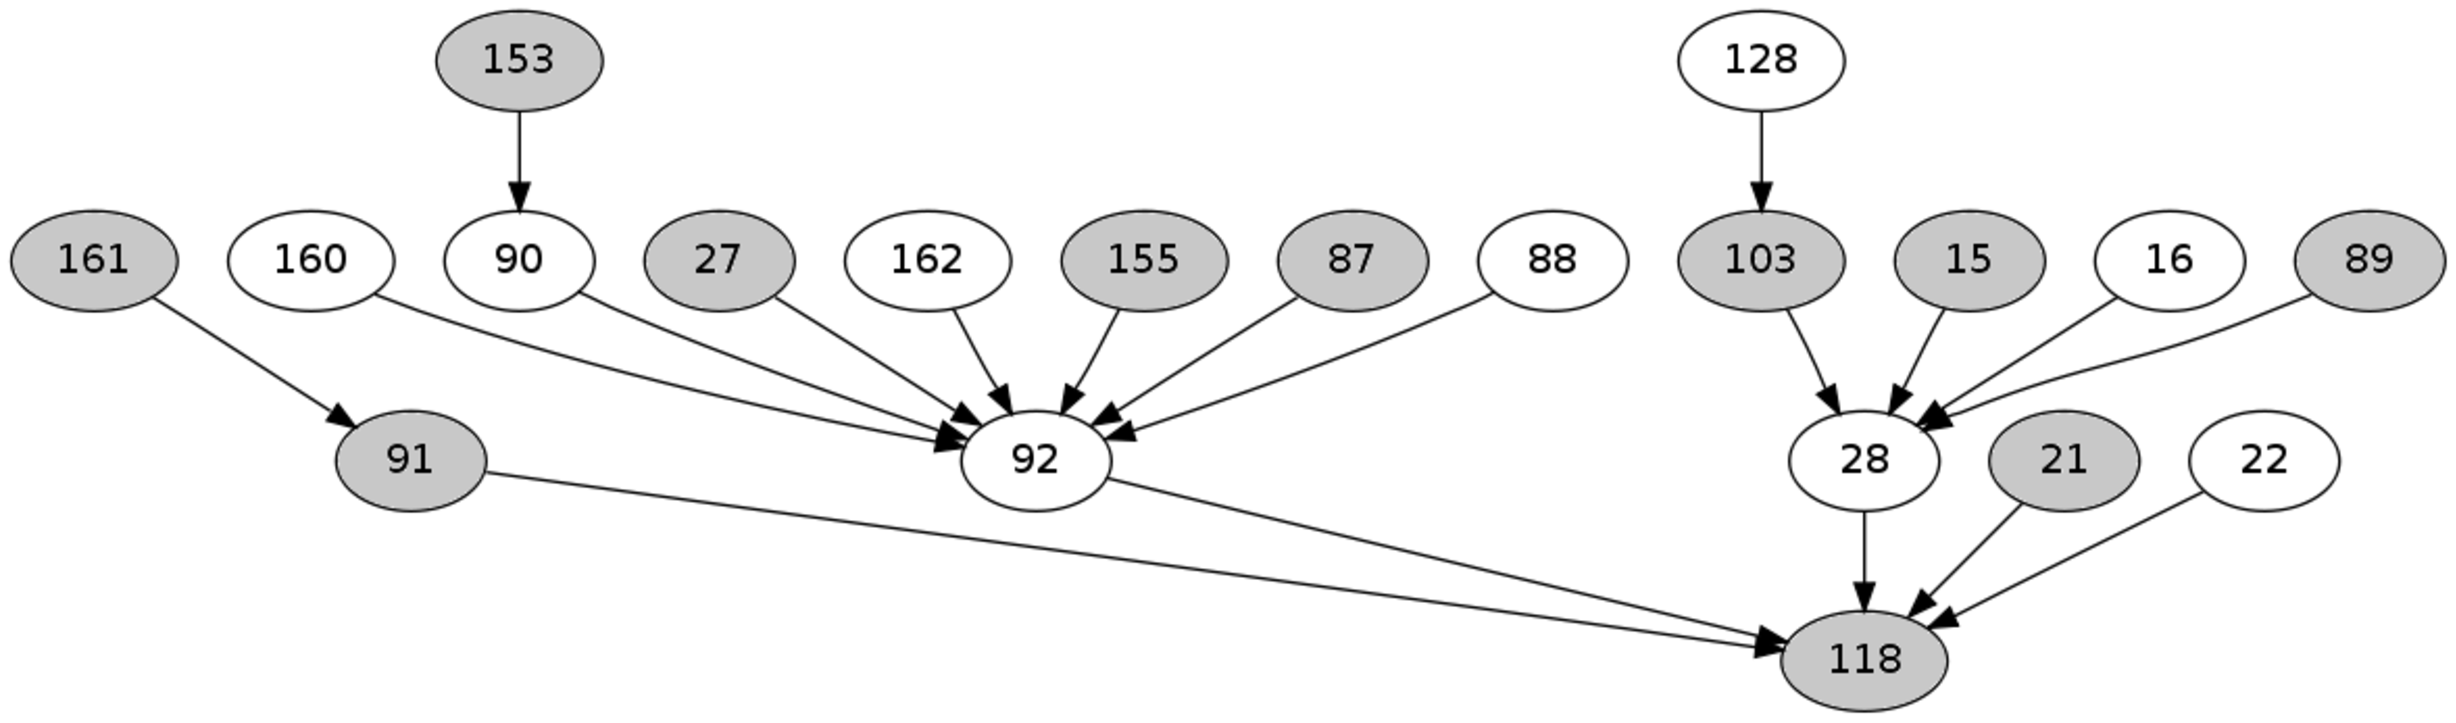
\includegraphics[width=0.7\hsize]{./5-idea/figs/ctp.pdf}\\
\textbf{(b)}\\
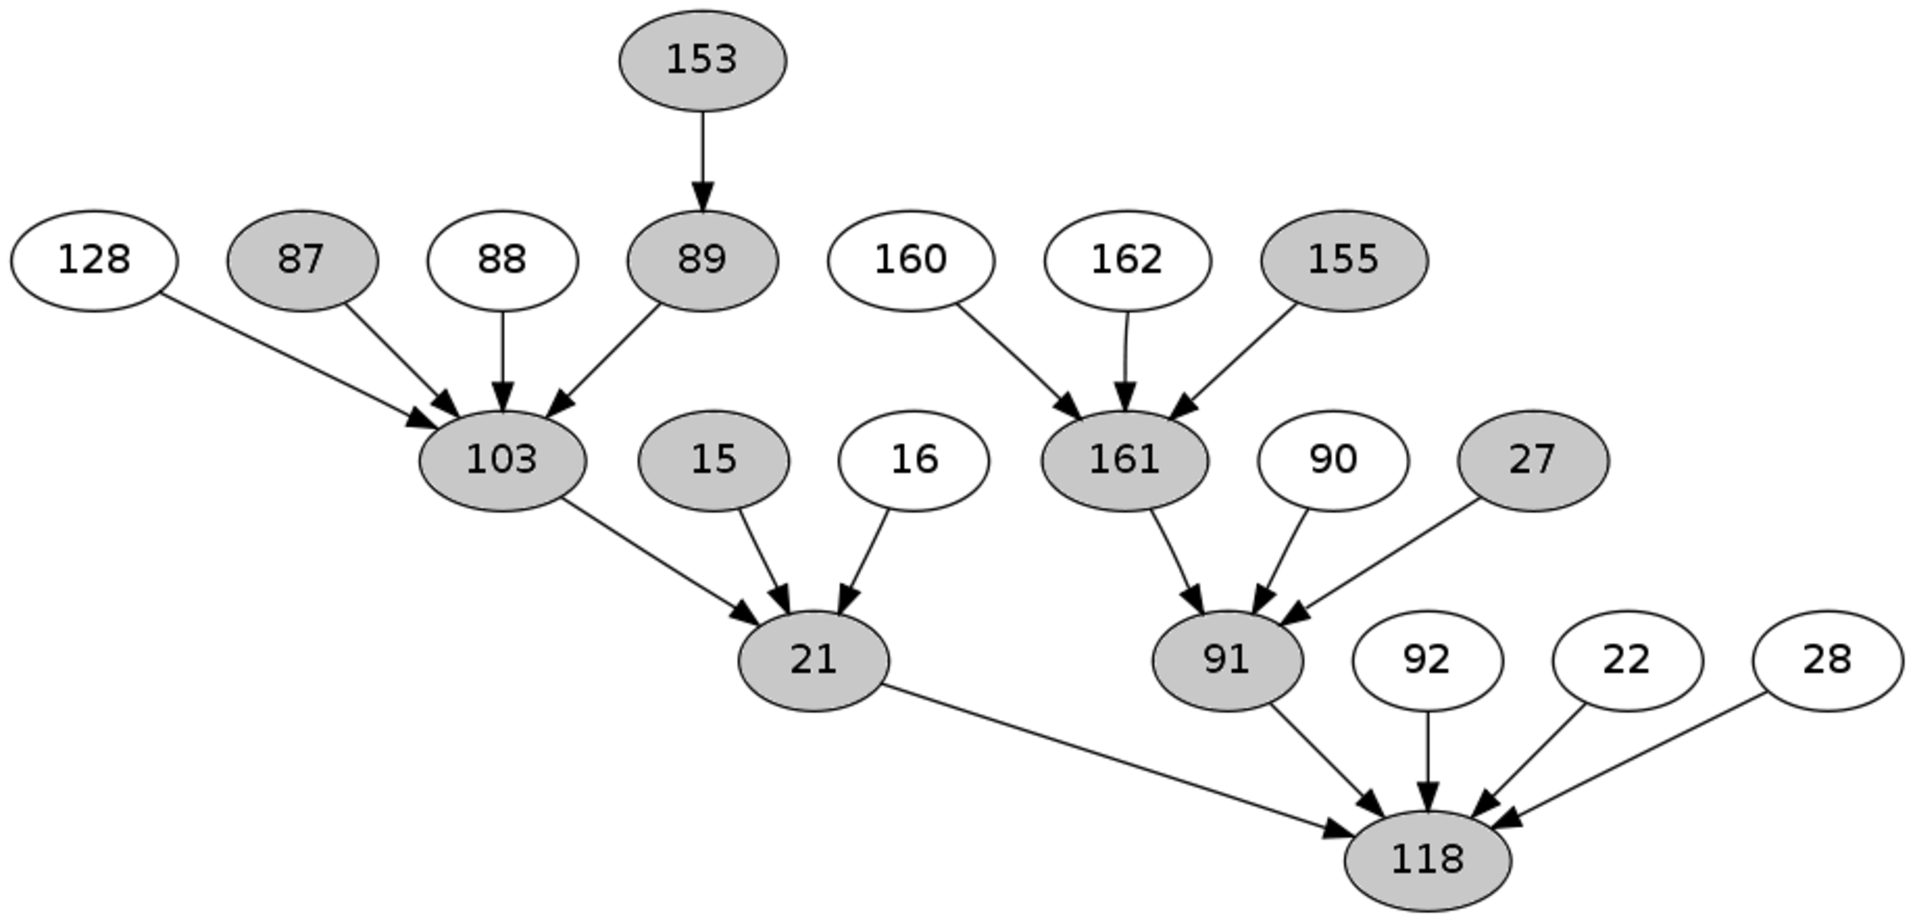
\includegraphics[width=0.7\hsize]{./5-idea/figs/ictp.pdf}\\
\end{center}

\caption{\textbf{Qualitative comparison of stock CTP and ICTP.} For this
experiment odd-numbered nodes (shaded) were set to charging rapidly, while
even-numbered nodes were not charging. Unmodified CTP builds the tree shown
in (a), which routes many packets through the even nodes. ICTP builds the
tree shown in (b), which moves all even nodes to leaf roles.}

\label{idea-fig-ictpqualitative}
\end{figure}

Using IDEA we were able to integrate energy awareness into CTP, the routing
protocol included as part of TinyOS. For these experiments each node in a
20~node network sends 6 packets to the sink per second. Static LPL intervals
of 0.5 second were used. 

Figure~\ref{idea-fig-ictpqualitative} shows a qualitative demonstration of
the difference between energy-aware and non-energy-aware routing trees. This
TOSSIM simulation ran with all odd numbered nodes charging rapidly and all
even numbered nodes not charging (with the exception of the powered sink,
Node 118). While this is an unrealistic charging pattern, it produces a clear
difference in routing protocol behavior.
Figure~\ref{idea-fig-ictpqualitative}(a) shows that unmodified CTP is unaware
of these charging differences and puts several even nodes, such as Node 92,
into positions where they are routing for multiple nodes. The total number of
nodes upstream from even numbered nodes in the stock CTP case is 14. In
contrast, ICTP realizes that the odd-numbered nodes have energy to spare and
the even-numbered nodes are lacking, and moves all even nodes to leaf roles.
None of the even nodes in Figure~\ref{idea-fig-ictpqualitative} are routing
data.

Using a 20~node subset of our MoteLab topology, we compared the performance
of ICTP to unmodified CTP using 24-hour TOSSIM simulations and the three
different solar charging scenarios previously described. As
Table~\ref{idea-table-ictpvoptimaltossim} shows, ICTP shows improvements in
lifetime over stock CTP of between 11 and 27\%. The different routing trees
formed by ICTP did not effect the packet delivery rates appreciably with the
largest change in packet delivery rate being 2.8\% (97.8\% for CTP vs. 95.0\%
for ICTP).

Finally, Table~\ref{idea-table-etxsearchradius} shows how IDEA can trade off
application utility with the energy objective function. The simulation
experiment uses a 25~node grid topology and, similar to the previous
experiment, half the nodes are charging rapidly while the other half are not.
Here our application-defined metric is expected transmissions to reach the
sink (ETX). A purely ETX-based tree will use the shortest route without
routing around the uncharging nodes, whereas an energy-aware tree will avoid
the uncharging nodes by constructing longer routes. We expect that,
prioritizing ETX will cause the total ETX of the entire tree --- defined as
the sum of the ETX of all the routes in use --- to decrease, while
prioritizing energy performance will cause the first-node lifetime of the
tree to increase.

Indeed, Table~\ref{idea-table-etxsearchradius} confirms this is the case. For
each experiment, we restrict the set of acceptable parents to be the minimum
available parent ETX plus an extra amount we call the ETX search margin. For
example, if the minimum available parent ETX is 5 and the ETX search margin
is 10, then we will consider all parents with ETX < 15. As the search margin
increases, IDEA will examine longer routes that may provide better energy
performance. As the table shows, increasing the ETX search margin leads to
longer average routes but also improves overall network lifetime.

\begin{table}[t]
\begin{center}
\begin{tabular}{|l|ccc|}
\hline
\textbf{Solar Charging} & \multicolumn{2}{c}{\textbf{Lifetime (hours)}} & \textbf{Increase} \\
\textbf{Pattern} & \textbf{CTP} & \textbf{ICTP} & \textbf{(\%)} \\ \hline
Large Panel & 17.1 & 19.0 & 11\% \\
Small Panel & 10.5 & 13.3 & 27\% \\
Random Attenuation & 10.5 & 12.2 & 16\% \\ \hline
\end{tabular}
\end{center}

\caption{\textbf{ICTP performance with solar charging.} The table summarizes
the performance improvements obtained by replacing CTP with ICTP. Three
different solar charging profiles are used: a large panel that completely
charges all batteries each day, a small panel that does not, and a randomly
attenuated charging profile that varies node-to-node.}

\label{idea-table-ictpvoptimaltossim}
\end{table}

\begin{table}[t]
\begin{center}
\begin{tabular}{|l|cc|}
\hline
\textbf{ETX Search} & \textbf{Total ETX} & \textbf{Network Lifetime} \\
\textbf{Margin (ETX)} & \textbf{(ETX)} & \textbf{(sec)} \\ \hline
0 & 2442 & 4357 \\
10 & 2591 & 4737 \\
20 & 3207 & 5116 \\
50 & 3127 & 6216 \\
100 & 3442 & 6502 \\ \hline
\end{tabular}
\end{center}

\caption{\textbf{Tradeoff between energy-awareness and application utility.}
The results illustrate how IDEA can parameterize the tradeoff between
application-defined utility and the energy objective function.}

\label{idea-table-etxsearchradius}
\end{table}

\subsection{Distributed Localization}

To evaluate the distributed localization application we built a Python
simulator, which improves significantly on TOSSIM performance for hundreds of
nodes and allowed rapid iteration and experimentation with different energy
objective functions. Our simulator models acoustic event sources within the
sensor network, each of which triggers a distributed localization operation.
The energy overheads of communication, both the leader election process and
the subsequent data transfer, are modeled in the simulator based on empirical
measurements taken on our MoteLab testbed.

\begin{figure}[t]
\begin{center}
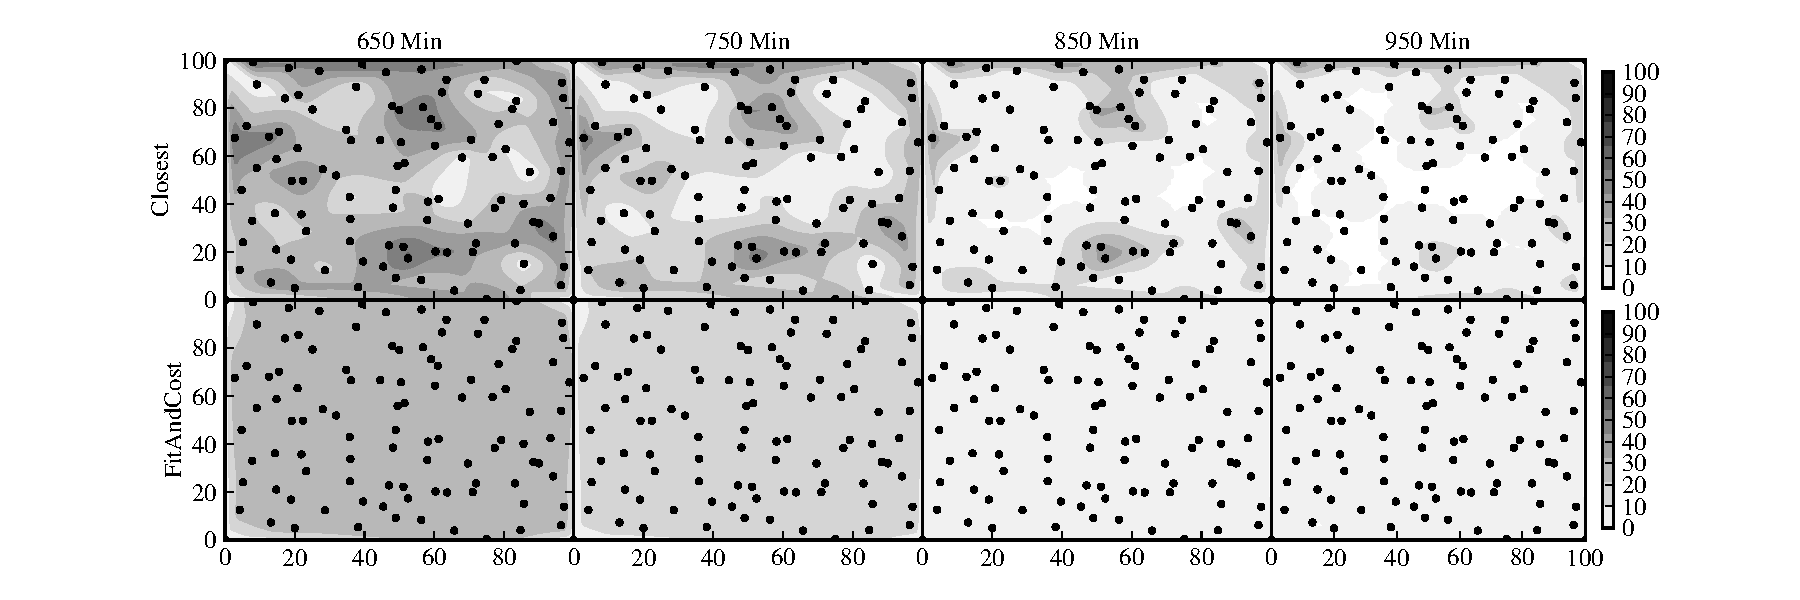
\includegraphics[width=\hsize]{./5-idea/figs/localizationdensityvtime.pdf}
\end{center}

\caption{\textbf{Energy density over time.} Energy densities for the
\texttt{Closest} heuristic and IDEA using the \texttt{WeightedEnergy}
objective function are shown at four points in time. The event distribution
is uniform. IDEA enables better load distribution, which leads to a longer
application lifetime.}

\label{idea-fig-localizationdensityvtime}
\end{figure}

For these experiments we arranged 100 nodes into a 100~m by 100~m area,
resulting in the placements shown in
Figure~\ref{idea-fig-localizationdensityvtime}. We simulate a sensing range
equal to the communication range, each set to 20~m. This radius is chosen to
give each node reasonable number of neighbors and allow it to detect a
reasonable number of events. We randomize the reliable transfer protocol
bandwidth across each link to between 768 and 1280~bytes/sec, a feasible
range based on results from data transfer protocols such as
Flush~\cite{flush-sensys07} and Fetch. Events are simulated using a uniform
random distribution so that events have equal probability of occurring
anywhere in the sensor field.

To evaluate network performance, we define \textit{capability} of the network
as the percent of the last 100 operations that succeeded, where success is
defined as localizing the event. We assume that the application requires that
the network be able to be able to localize a high percentage of events that
occur, and design our energy objective functions with this in mind. As an
example, an intruder localization application is no longer useful once it
fails to detect a very high percentage of intrusion attempts. We quote the
system lifetime as the the 90\% capability time, the time at which the
network's capability drops below 90\%.

We experimented with several approaches to choosing a localization plan, one
that does not use IDEA and three that do using different energy objective
functions:

\begin{enumerate}

\item \textbf{\texttt{Closest}:} produces a localization plan with the node
closest to the event source as the aggregator and the three next closest
nodes as signal providers. We assume a real solution would use an imperfect
estimate of proximity such as total signal energy or signal-to-noise ratio,
but for the simulations we use the known simulated event location to choose
the closest nodes. \texttt{Closest} does not require energy state information
and so could be implemented without IDEA. It is implemented as an example of
a plausible non-energy-aware solution.

\item \textbf{\texttt{MaxEnergy}:} chooses the node with the most energy
(that heard the event) as aggregator and the next three highest-energy nodes
as signal providers.

\item \textbf{\texttt{TotalEnergy}:} chooses the localization plan that
consumes the lowest amount of total energy summed across all nodes in the
network.

\item \textbf{\texttt{WeightedEnergy}:} weights the total energy consumption
using a similarity metric derived from the cosine similarity index to measure
the degree to which the energy vector for the localization plan is a good
``fit'' given the current energy availability.

\end{enumerate}

\begin{figure}[t]
\begin{center}
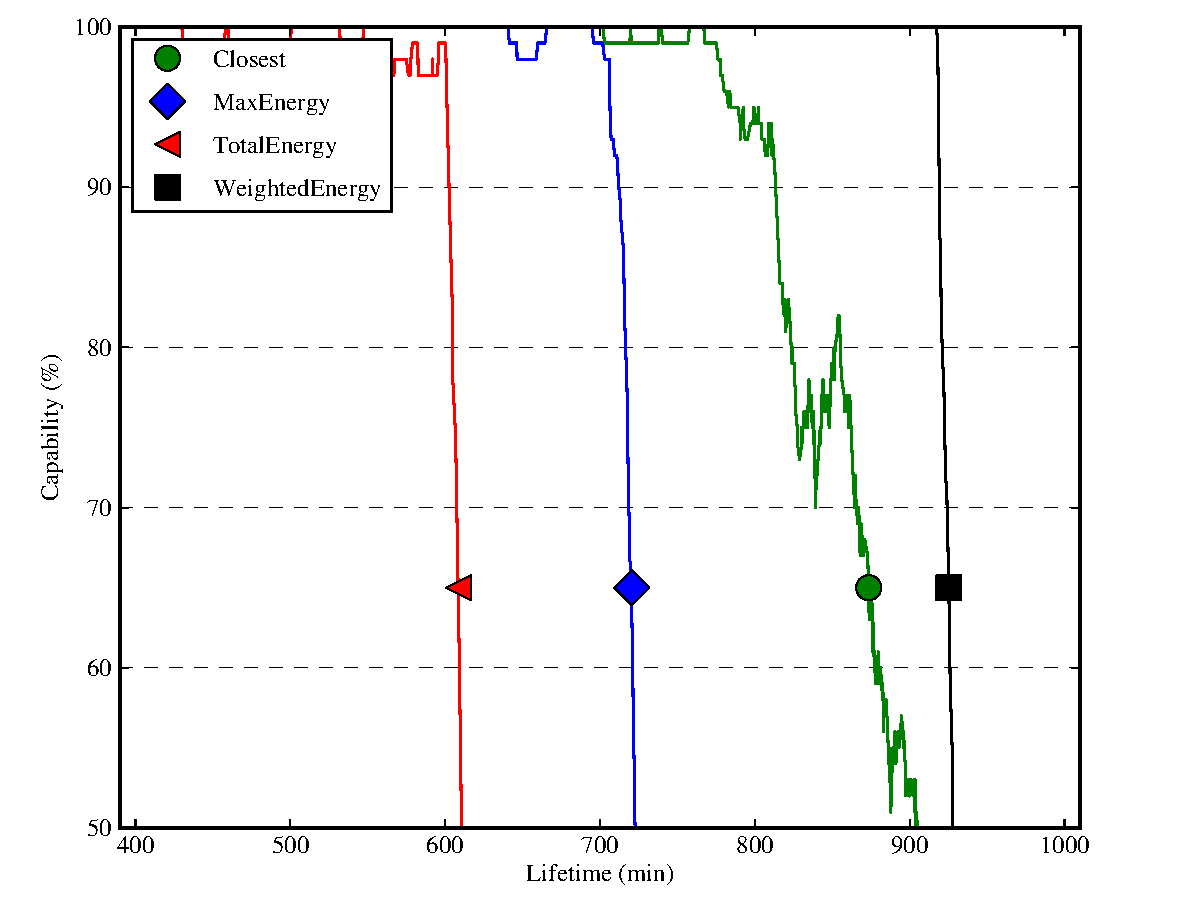
\includegraphics[width=0.7\hsize]{./5-idea/figs/ideavheuristics.pdf}
\end{center}

\caption{\textbf{Performance of IDEA objective functions and heuristic.}
Simulation results are shown for the localization application. The graph
compares the \texttt{Closest} heuristic, implemented without using IDEA,
against three different IDEA objective functions: \texttt{MaxEnergy},
\texttt{TotalEnergy} and \texttt{WeightedEnergy}. The \texttt{WeightedEnergy}
approach using IDEA outperforms the non-energy-aware approach while the other
objective functions perform more poorly.}

\label{idea-fig-ideavheuristics}
\end{figure}

We began by experimenting with the \texttt{Closest}, \texttt{MaxEnergy} and
\texttt{TotalEnergy} approaches. As Figure~\ref{idea-fig-ideavheuristics}
shows, the \texttt{Closest} heuristic outperformed the two IDEA-based
approaches. However, when examining the energy density plot shown in
Figure~\ref{idea-fig-localizationdensityvtime} for the \texttt{Closest}
heuristic we could see that it led to concentrations of available energy on
nodes at dense locations on the irregular grid, while \texttt{MaxEnergy} did
a better job of exhausting all nodes simultaneously, as evidenced by the
extremely sharp drop in network capability it produces. This is despite the
uniform distribution of acoustic event sources, which one might expect to
produce good energy load distribution without the need for tuning.

Our analysis determined that the \texttt{MaxEnergy} suffers because it will
always route data through extra nodes in order to reach the node with the
most energy. So if that node is on the edge of the cluster of nodes that
heard the event, energy may be consumed by nodes within the interior in order
to allow the signal provides to communicate with the aggregator.
\texttt{MaxEnergy} leads to an even usage of energy across the network, but a
short lifetime, because it always prioritizes the distribution of energy over
the amount consumed when choosing how to localize each event.

In contrast, \texttt{Closest}, while it performs better, has the opposite
problem. While it does not consider energy directly, the effect of the
heuristic is to choose based on the total amount of energy consumed. By
selecting the nodes closest to the event, the heuristic almost always leads
to clusters where all signal providers can communicate with the aggregator,
so no extra energy expenditures by other nodes for routing are needed.
However, the non-uniform distribution of nodes means that some nodes more
likely to be the closest node than others, leading to unequal energy
distribution. While the lifetime is better than \texttt{MaxEnergy}, the
existence of energy at some nodes once the capability drops below 90\% led us
to believe that a hybrid approach was possible that would outperform both
\texttt{MaxEnergy} and \texttt{Closest}.

After exploring several additional approaches we found an energy objective
function capable of producing extremely good load distribution, the
\texttt{WeightedEnergy} approach described above.
Figure~\ref{idea-fig-ideavheuristics} shows that it outperforms
\texttt{Closest}, increasing the network's lifetime by 15\%, while
Figure~\ref{idea-fig-localizationdensityvtime} illustrates how it utilizes
all the nodes' available energy, achieving an even distribution similar to
\texttt{MaxEnergy}. It does this by combining aspects of both earlier
approaches. By weighing the total energy consumed it avoids the extremely
high-energy localization plans that the \texttt{MaxEnergy} function will
sometimes use. By also weighing the ``fit'' using the cosine similarity
metric we address unequal energy distribution in a way that the
\texttt{Closest} heuristic does not.

Our experience with the localization application illustrates the role of the
proper energy objective function in enabling good application performance,
and points to the increases in system lifetime possible through better energy
distribution. 

\section{Field Deployment at Tungurahua Volcano}
\label{lance-sec-deployment}

To evaluate the performance of Lance in a real field setting, we undertook a
one week deployment of eight~sensor nodes at Tungurahua Volcano, Ecuador, in
August~2007. Lance was used to manage the bandwidth resources of the sensor
network, as described below. Time and budget constraints prevented us from
deploying a larger network for longer period of time. An earlier version of
Lance was used in this deployment that did not explicitly model energy cost
in the download manager. However, due to the short duration of the
deployment, we knew that the battery lifetime used would be more than
adequate (two D-cell batteries offer a lifetime of approximately 12~days with
this platform). Our primary goal was to validate Lance's operation in a field
campaign, as well as to identify challenges that only arise in real
deployments.

\begin{figure}[t]
\begin{center}
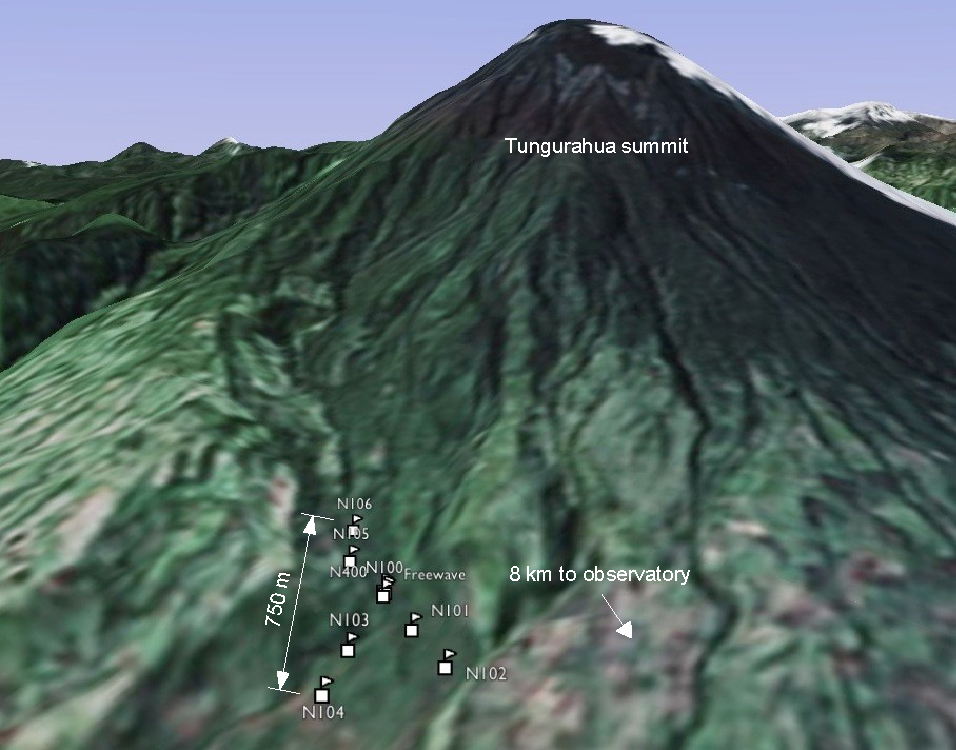
\includegraphics[width=0.7\hsize]{./4-lance/figs/map.pdf}
\end{center}

\caption{\textbf{Location of the Tungurahua sensor network deployment.}}

\label{lance-fig-map}
\end{figure}

As shown in Figure~\ref{lance-fig-map}, seven of the nodes were deployed in a
three-armed ``star'' topology radiating away from a central hub node, with
two nodes per arm. The eighth node was colocated with the hub and transmitted
an unreliable continuous stream of sensor data packets for establishing
ground truth. A separate gateway node relayed data (using a FreeWave radio
modem) to the base station laptop at the volcano observatory, 8~km from the
deployment site. Time synchronization was established using FTSP~\cite{ftsp}
with a single GPS receiver as the root of the synchronization tree. We
experimented with two different summarization functions as well as several
different policy modules during the field deployment.

\subsection{Overall Performance and Data Yield}

\begin{figure}[t]
\begin{center}
\begin{tabular}{|l|l|l|} \hline
\textbf{Node}	& \textbf{ADUs downloaded} & \textbf{Mean throughput} \\ \hline
100 & 311 & 651.0 Bps \\
101 & 131 & 446.8 Bps \\
102 & 262 & 445.8 Bps \\
103 & 292 & 424.4 Bps \\
104 & 150 & 256.8 Bps \\
105 & 66 & 453.7 Bps \\
106 & 20 & 253.4 Bps \\ \hline
\textit{Total} & 1232 & 431.5 Bps \\ \hline
\end{tabular}
\end{center}

\caption{\textbf{Download performance during the deployment.}}

\label{lance-fig-throughput}
\end{figure}

The sensor network was operational for a total of 71~hours, out of which the
Lance download manager ran for a total of 56~hours. During this time, Lance
successfully downloaded 1232~ADUs, or 77~MB of raw data. An additional
308~downloads failed due to timeout or stale summary information, for an
overall success rate of 80\%. 11012~unique ADU summaries were received from
the network, representing an aggregate of 688~MB of sampled data. Lance
therefore downloaded approximately 11\% of the data produced by the network.
Figure~\ref{lance-fig-throughput} summarizes the number of ADUs downloaded
and the mean throughput for each node.

\begin{figure}[t]
\begin{center}
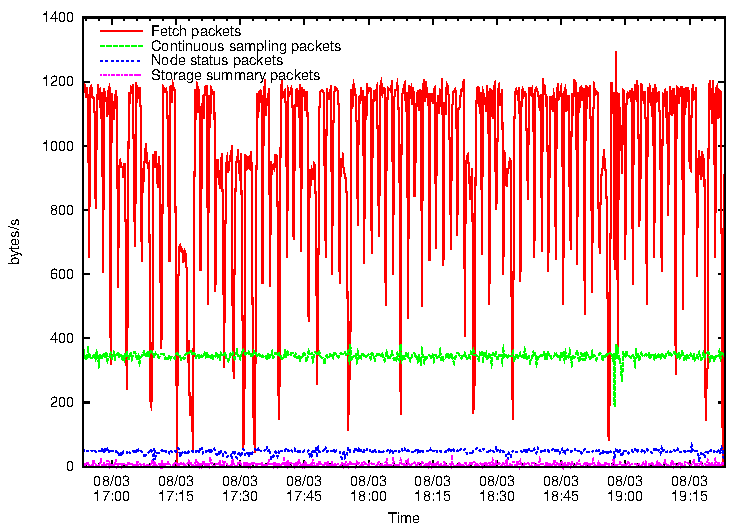
\includegraphics[width=0.9\hsize]{./4-lance/figs/packetgraph.pdf}
\end{center}

\caption{\textbf{Breakdown of radio traffic by packet type.} This figure
shows the total number of bytes received at the base station, averaged over
15~s intervals. Periodic node status messages and storage summaries comprise
a small fraction of the overall bandwidth.}

\label{lance-fig-packetgraph}
\end{figure}

Figure~\ref{lance-fig-packetgraph} shows a breakdown of the packets received
at the base station for a representative time period. Fetch download packets
consumed the majority of the bandwidth, followed by the continuous sampling
packets. The latter is a debugging feature allowing us to visualize the
seismic activity from a single node in real time, and is entirely optional.
Every node sent a periodic heartbeat to the base station every~10~s, and a
storage summary every 109~s. As the figure shows, this overhead is a small
percentage (less than 5\%) of the overall network traffic.

\subsection{RSAM-based Summarization}

\begin{figure}[t!]
\begin{center}
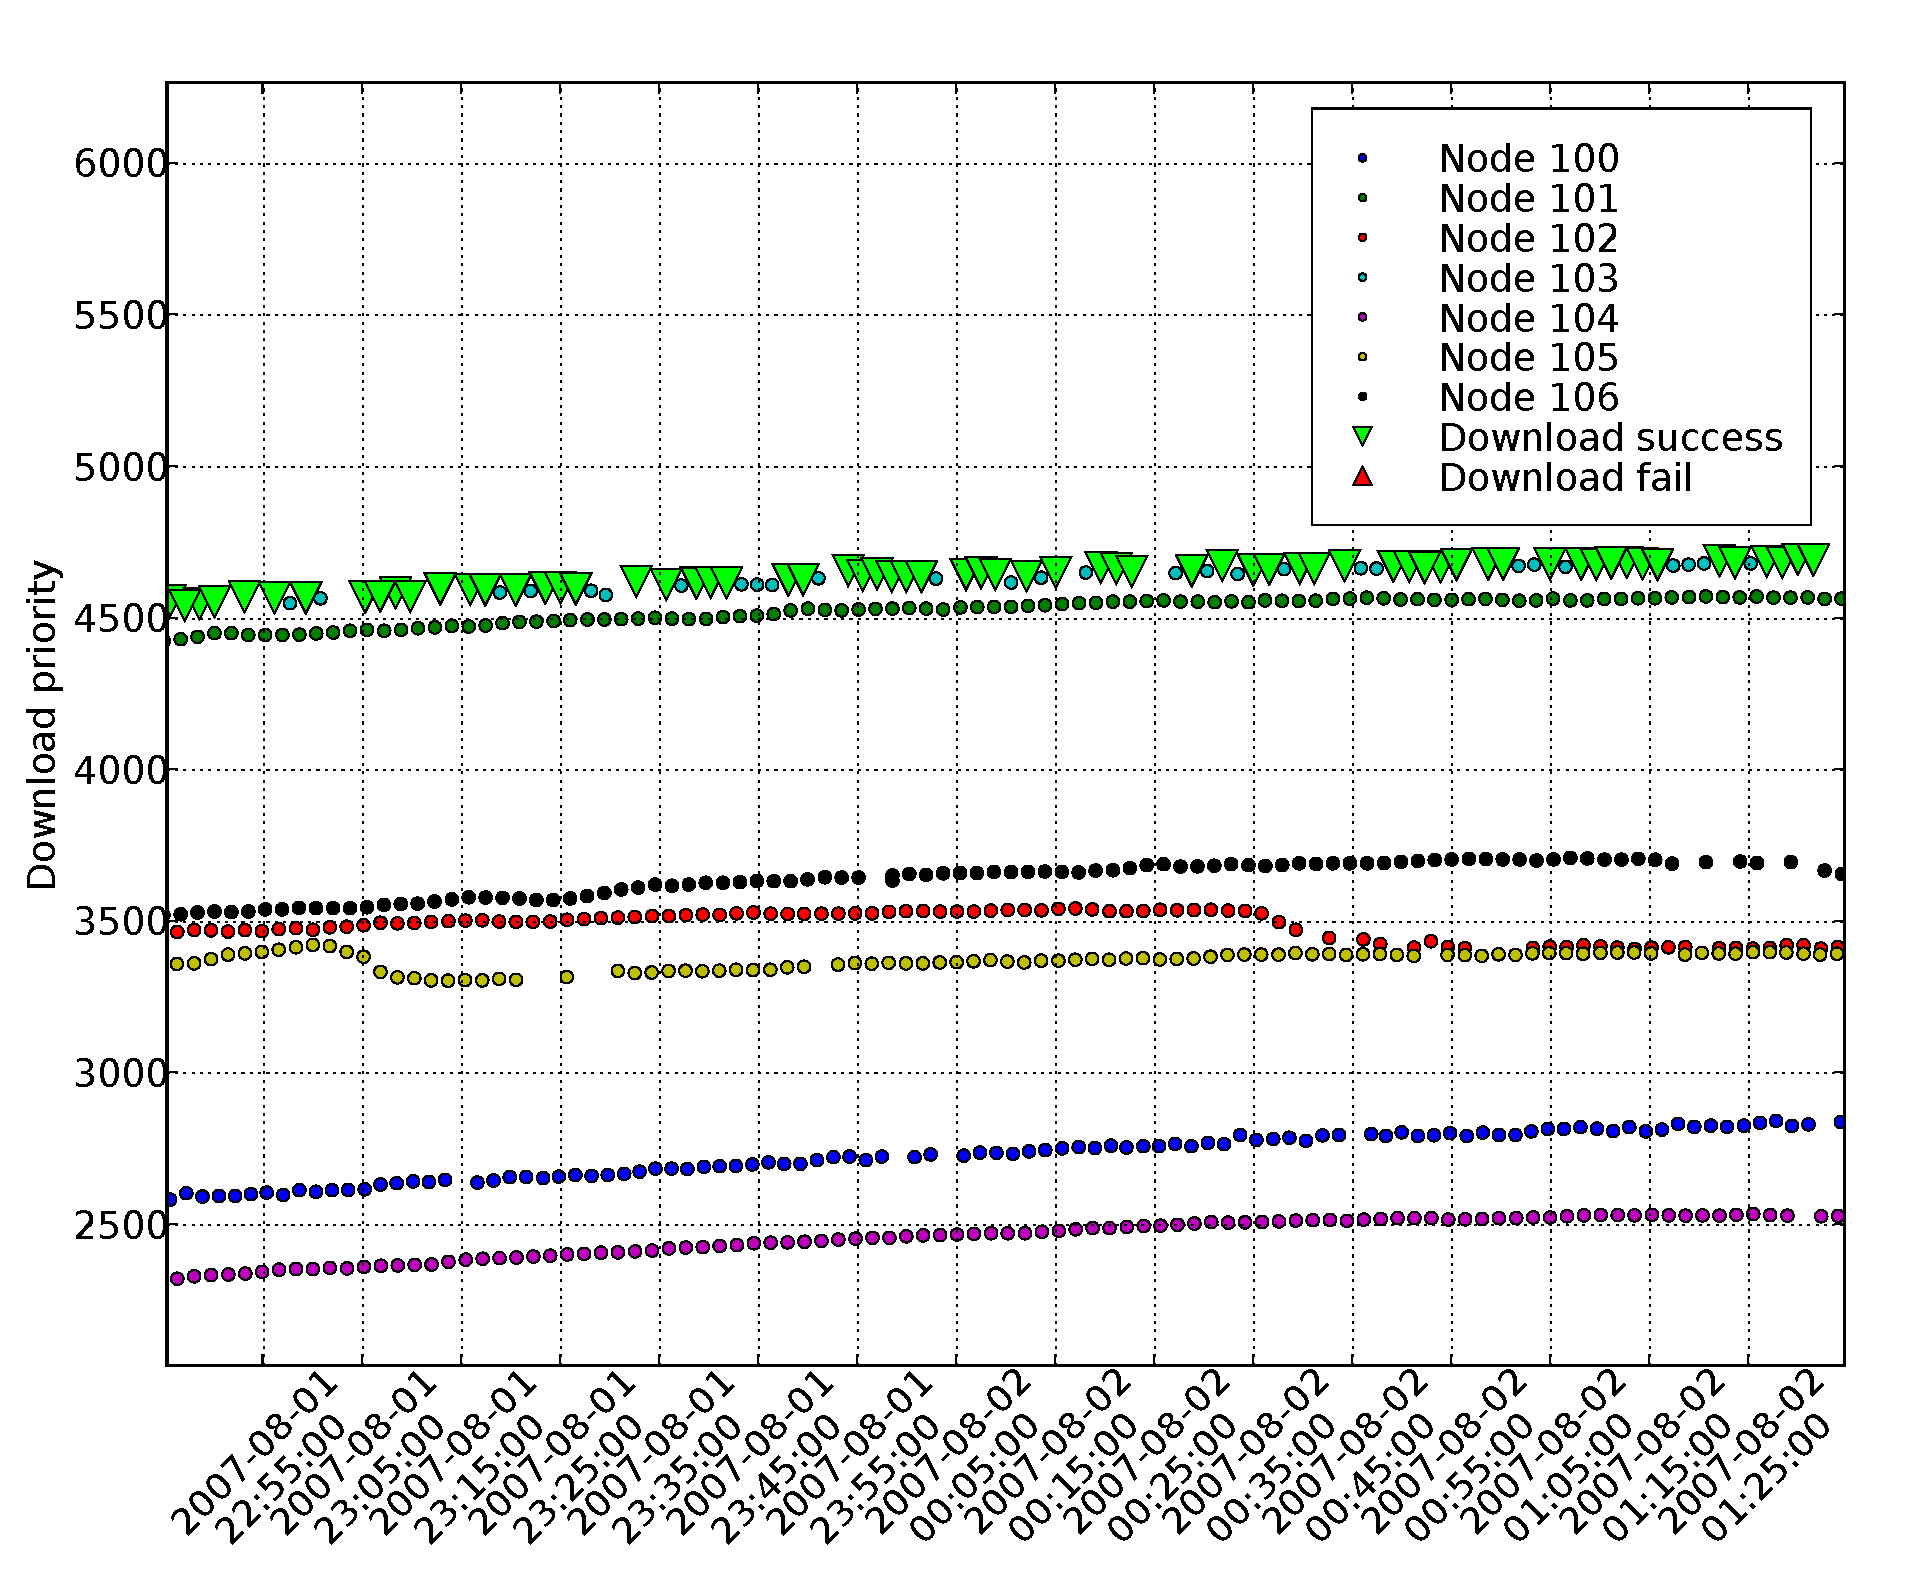
\includegraphics[width=0.8\hsize]{./4-lance/figs/dcbias.pdf}
\end{center}

\caption{\textbf{Effect of DC bias on RSAM summarization function.} Each
point represents the ADU value received at the base station, and the
triangles indicate those ADUs that were downloaded by Lance. Since nodes'
RSAM values are offset significantly from each other, Lance prefers
downloading from the node with the largest positive bias.}

\label{lance-fig-dcbias}
\end{figure}

The system as initially deployed computed the RSAM~\cite{rsam} as the value
for each ADU. This approach was intended to prioritize data based on the
overall level of seismic activity. We experienced two problems as soon as the
system was fielded. First, the RSAM calculation was sensitive to DC~bias in
the seismometer signal, causing Lance to generally prefer downloading ADUs
from one or two nodes (those with the largest positive bias).
Figure~\ref{lance-fig-dcbias} shows this effect, with Lance only downloading
ADUs from Node~103.

This problem was easily corrected, without any node software changes, by
introducing a policy module at the base station to process the raw RSAM
values received from each node and filter out the DC~bias. This was achieved
by computing the median RSAM value over each 30-minute window of raw RSAM
values on each node, and subtracting the median from the RSAM.

The second problem with the RSAM summarization function was caused by the
uncharacteristically low level of seismicity at the volcano throughout the
deployment. We observed only about 20~volcano-tectonic earthquakes and
\textit{no} clear explosions, whereas the previous week, Tungurahua exhibited
dozens of earthquakes each day. As a result, the RSAM summarization function
was generally unable to distinguish between actual seismic activity and
noise. We corrected this problem by switching to a different summarization
function (described below) that was designed to pick out small earthquakes.

To evaluate Lance's behavior with respect to an ``optimal'' system, we took
the 8483~RSAM summaries received during a 16-hour period when the debiasing
filter was enabled. Using this information, we compute the set of ADUs that
the optimal system would have downloaded, with complete knowledge of all ADUs
but limited to the same time duration the original network was operating. We
assume the download throughput for a given node is always the mean throughput
for that node observed during the deployment
(Figure~\ref{lance-fig-throughput}). This calculation ignores energy
constraints because the deployed system did not consider energy costs.

An optimal system would have downloaded 392~out of the~8483 ADUs, whereas the
actual system downloaded 418~ADUs during this time.\footnote{The optimal
system would download fewer ADUs than the real system due to the variation in
the throughput to each node: the optimal system would download more ADUs from
nodes with lower throughput, thereby limiting the total number of ADUs it
could download.} The total value of ADUs downloaded by the optimal system is
10678, whereas the value of the actual network was 10629, for an optimality
of 99.5\%. Lance did an exceptional job of extracting the highest-value data
from the network using our online heuristic algorithm.

\subsection{EWMA-based Summarization Function}
\label{lance-sec-ewma-deployment}

Given the low level of volcanic activity, after the first 25~hours of the
deployment we chose to reprogram the network to use a different summarization
function that is designed to pick out small earthquakes from background
noise. This function computes the maximum ratio of two EWMA filters over the
seismic signal; it is similar to that described in~\cite{volcano-osdi06}. Due
to code size limitations on the motes, it was necessary to manually reprogram
each node with the new summarization function, which took two teams about
4~hours.

This summarization function reports a high value for an ADU that appears to
contain an earthquake or other seismic event. However, there is no guarantee
that the event will be centered in the ADU: in the worst case, the earthquake
might occur at the very beginning or very end of the ADU, causing the initial
seismic P-wave arrival or waveform coda to be stored in adjacent ADUs with
low value. To avoid this problem, we made use of the \texttt{timespread}
policy module that detects ADUs with an elevated value (over a fixed
threshold) and assigns the immediately preceding and succeeding ADUs the same
value. By dilating the value over time, Lance should download all three of
the ADUs and maximize the probability that a given earthquake signal is
entirely downloaded.

As with the RSAM-based summarization function, we estimate the optimal set of
ADUs that an oracle would have downloaded. During a 25-hour period, the
network reported 11012~unique ADU summaries. An optimal system would have
downloaded 554 ADUs with total value 577377. The actual network downloaded
518~ADUs with a value of 539115, for an optimality of 93.3\%.

As a final evaluation metric, we wish to consider how well Lance, configured
in this manner, was able to download seismic signals representing
earthquakes. Given the low level of volcanic activity, it turns out that most
of the ADUs downloaded by Lance contain no discernible seismic signal. In
fact, upon manual inspection of the 518~ADUs downloaded during this period,
we identified only 20~ADUs showing a clear earthquake signal, corresponding
to only 9~separate seismic events. Note that we did \textit{not} configure
Lance to explicitly download correlated earthquakes as described in
Section~\ref{lance-sec-adaptation} so we would not expect a high degree of
coverage for the same event across multiple nodes.

\begin{figure}[t]
\begin{center}
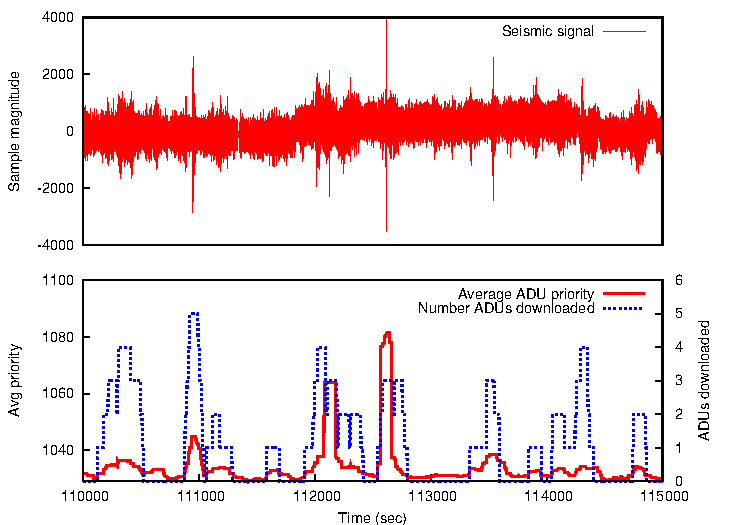
\includegraphics[width=1.0\hsize]{./4-lance/figs/everything.pdf}
\end{center}

\caption{\textbf{Lance download behavior overlayed with average ADU value.}
The top plot shows the continuous seismic signal collected by a single node.
The lower plot shows the average value of ADUs and the number of ADUs
downloaded for each window.}

\label{lance-fig-everything}
\end{figure}

Figure~\ref{lance-fig-everything} shows the behavior of Lance during a
representative 83-minute period. In the figure, we have broken time into
windows of one-half an ADU duration (55~s in this case), and computed the
mean ADU value as well as the number of downloaded ADUs that overlap each
time window. As the data shows, elevated seismic activity is well-correlated
with an increase in the ADU value from across the network, as well as the
number of downloaded ADUs. Moreover, the few cases of clear seismic activity
in the trace (at times 111000, 112700, and so forth) tend to have more ADUs
downloaded. Of the 9~separate seismic events, a total of 27~ADUs were
downloaded, representing a per-event ``coverage'' of 3~ADUs per event. This
represents just under half of the 7~nodes participating in the network.

\section{Conclusions}
\label{sec-conclusions}


%%%%%%%%%%%%%  THIS IS WHERE THE BIBLIOGRAPHY GOES %%%%%%%%%

%\def\baselinestretch{0.92}
%\begin{footnotesize}
%\setlength{\itemsep}{1in}
\bibliographystyle{abbrv} \bibliography{sensys08}
%\end{footnotesize}

\end{document}
